\documentclass[a4paper, 15pt]{article}
\usepackage[left=0.85in, right=0.85in, top=0.5in, bottom=0.95in]{geometry}
\usepackage[T1]{fontenc}
\usepackage[utf8]{inputenc}
\usepackage[italian]{babel}

% Formattazione del testo
\usepackage{setspace}         % Setting dello spazio\begin{spacing}{0.95}
	\setstretch{1.2}
	\setlength{\parindent}{0pt}
	\raggedbottom
	\usepackage[none]{hyphenat}    % no sillabazione 
	\usepackage{multicol}          % testo su più colonne
	\usepackage{changepage, float}	       % \begin{adjustwidth}{}{}
		
		% Matematica
		\usepackage{amsmath, amssymb, amsthm, mathtools}
		\usepackage{cancel}            % semplificazioni \cancel{expression}
		\newtheorem*{thm}{Teorema}
		\newtheorem*{en}{Enunciato}
		\newtheorem*{definizione}{Definizione}
		\newtheorem*{cor}{Corollario}
		\DeclareMathOperator{\rk}{rk}
		\DeclareMathOperator{\im}{Im}
		
		% Simboli e Disegni
		\usepackage{color}             % \textcolor{'ColorCode'}{'testo'}
		\usepackage{graphicx, wrapfig}
		\usepackage{tikz, circuitikz}
		\usetikzlibrary{patterns, arrows, decorations.markings, arrows.meta, decorations.text}
		\tikzset{immagine/.style={above right, inner sep=0pt, outer sep=0pt},
			testo/.style={fill=white, align=center, fill opacity=0.6, text opacity=1, below, font=\sffamily\bfseries\footnotesize}}
		\usepackage{pgfplots}
		\pgfplotsset{compat=1.15}
		\usepackage{mathrsfs}
		
		% Altri pacchetti
		\usepackage{enumitem}
		\usepackage{mdwlist} 	       % suspend enumerate \suspend{} \resume{}
		\usepackage{siunitx}
		\usepackage{hyperref}
		\hypersetup{
			colorlinks=true,
			linkcolor=blue,    
			urlcolor=blue,
		}
		\urlstyle{same}
		
		% Altre definizioni personali
		\usepackage{pifont}
		\newcommand{\cmark}{\ding{51}}
		\newcommand{\xmark}{\ding{55}}
		\DeclareUnicodeCharacter{20AC}{\EUR}
		\newcommand{\compresslist}{\setlength{\itemsep}{1pt}\setlength{\parskip}{0pt}\setlength{\parsep}{0pt}}
		\newcommand{\ra}[1]{\renewcommand{\arraystretch}{#1}} % stretcho le tabelle e gli array \ra{x}
		\setlength{\jot}{10pt}
		
		
		% Titolo e data
		\title{De Saint Venant}
		\date{}
		
		\begin{document}
			\maketitle
			\setcounterpageref{secnumdepth}{0}
			\setcounter{tocdepth}{5}  % Includo nel TOC anche i subsubpar	
			\tableofcontents 
			\newpage
			


	
\section{Il problema di De Saint Venant}	
	Il modello alla De Saint Venant si propone di ricavare deformazioni e tensioni su di un oggetto ideale, a partire dai carichi esterni opportunamente applicati. 
	
	Si ipotizzeranno delle soluzioni che sostituite nel problema porteranno al soddisfacimento delle ipotesi (metodo inverso): partendo dalle ipotesi di De Saint Venant, si ipotizzerà una soluzione, se questa sostituita nelle ipotesi di partenza le soddisferà, allora la soluzione sarà esatta, ed esistendo, per il principio di Kirchhoff, sarà l'unica. \newline
	
\subsection{Ipotesi semplificative}
\begin{figure}[H]
	\centering
	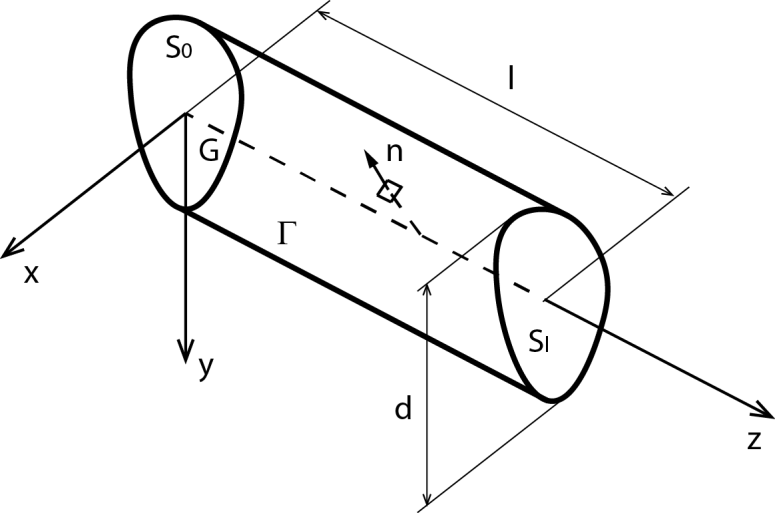
\includegraphics[width=0.5\linewidth]{Immagini_2/screenshot001}
	\label{fig:screenshot001}
\end{figure}
	\begin{enumerate}
	\item \textbf{Ipotesi sulla geometria}:
		\begin{itemize}		
		\item La dimensione caratteristica (ingombro massimo di sezione) della sezione retta della trave
		deve risultare trascurabile rispetto alla sua lunghezza $ d/l<<1 $: la trave dev'essere snella, non tozza;
		\item La trave è ad asse rettilineo;
		\item Sezioni rette costanti lungo z;
		\end{itemize}

	\item \textbf{Ipotesi sui carichi esterni}:
		\begin{itemize}
			\item  Le forze di volume $ f $ sono nulle, si ignora la forza peso;
		\item Le forze di superfici	$ p $ sono applicate solo sulle basi e non sulla superficie laterale;
		\item Il sistema si trova in equilibrio;
		\item Il corpo è libero da vincoli, trascuro ovvero i carichi da questi generati all'interno delle caratteristiche della sollecitazione;
		\end{itemize}
	\item \textbf{Ipotesi sul materiale costitutivo}:
		\begin{itemize}
			\item Materiale elastico lineare e isotropo (due parametri per caratterizzarlo: Young e Poisson);
		\item La trave è omogenea, ovvero le caratteristiche del	materiale non variano da punto a punto
		\end{itemize}
	\end{enumerate}
	Con un sistema di riferimento baricentrico con $z$ asse della trave. \newline 
	
	\textbf{Equazioni indefinite di equilibrio}:
\[ \text{in} ~ \Omega
\begin{cases}
	\begin{aligned}
		\frac{\partial\sigma_x}{\partial x} + \frac{\partial \tau_{yx}}{\partial y} + \frac{\partial \tau_{zx}}{\partial z} & =0 \\
		
		\frac{\partial \tau_{xy}}{\partial x} + \frac{\partial\sigma_y}{\partial y} + \frac{\partial \tau_{zy}}{\partial z} & =0 \\
		
		\frac{\partial \tau_{xz}}{\partial x} + \frac{\partial \tau_{yz}}{\partial y} + \frac{\partial\sigma_z}{\partial z} & =0 \\
	\end{aligned}
\end{cases}
\]

	\textbf{Equazioni al contorno:} 
\[
\text{in} ~ \Sigma \begin{cases}
	p_x = \sigma_x n_x + \tau_{yx}n_y + \tau_{zx}n_z \\
	p_y = \tau_{xy}n_x + \sigma_y n_y + \tau_{zy}n_z \\
	p_z = \tau_{xz}n_x + \tau_{yz}n_y + \sigma_z n_z \\
\end{cases}
\]
\[
\text{mantello} ~ (n_x,n_y,0) \begin{cases}
\sigma_x n_x + \tau_{yx}n_y =0 \\
\tau_{xy}n_x + \sigma_y n_y =0 \\
\tau_{xz}n_x + \tau_{yz}n_y =0 \\
\end{cases} 
\]
\[
\text{$S_0$} ~ (0,0,-1) ~ \begin{cases}
	\tau_{zx} = -p_x \\
	\tau_{zy} = -p_y \\
	\sigma_z = -p_z \\
\end{cases}
\hspace{0.5cm}
\text{$S_l$} ~ (0,0,1) ~ \begin{cases}
	\tau_{zx} = p_x \\
	\tau_{zy} = p_y \\
	\sigma_z = p_z \\
\end{cases}
\]

\textbf{Legame costitutivo:}
\[ [\varepsilon] = [C][\sigma]\]

	\textbf{Equazioni di congruenza:}
\[ 
\begin{cases}
	\begin{aligned}
		\varepsilon_{xx} =   \frac{\partial u_x}{\partial x} \\
		\varepsilon_{yy} =   \frac{\partial u_y}{\partial y} \\
		\varepsilon_{zz} =   \frac{\partial u_z}{\partial z} \\
	\end{aligned}
\end{cases} \hspace{1cm} \begin{cases}
	\begin{aligned}
		\gamma_{xy} =   \frac{\partial u_y}{\partial x} + \frac{\partial u_x}{\partial y} \\
		\gamma_{yz} =   \frac{\partial u_y}{\partial z} + \frac{\partial u_z}{\partial y} \\
		\gamma_{zx} =   \frac{\partial u_z}{\partial x} + \frac{\partial u_x}{\partial z} \\
	\end{aligned}
\end{cases}
\]
\begin{figure}[H]
	\centering
	\includegraphics[width=0.5\linewidth]{Immagini_2/screenshot002}
	\label{fig:screenshot002}
\end{figure}
Ottengo così un set di equazioni per cui si ipotizzerà una soluzione che si dovrà verificare in queste equazioni per controllare che siano tutte rispettate. \newline 

È necessario tradurre le sollecitazioni in tensioni: servono le caratteristiche della sollecitazione. 
\begin{itemize}
	\item[$\rightarrow$] La risultante dello \textbf{sforzo normale}? È la risultante delle azioni in direzione $z$; 
\item[$\rightarrow$] La risultante dello \textbf{sforzo di taglio}? È la risultante delle rispettive azioni sull'asse $x$ e sull'asse $y$
\item[$\rightarrow$] Come si genera il momento intorno all'asse $x$? $P_x$ e $P_y$ giacciono in $xy$ e quindi non hanno braccio per generare una rotazione intorno ad $x$, l'unica azione che può farlo è $P_z$.
\item[$\rightarrow$] Il \textbf{momento intorno all'asse $y$} sarà generato come appena detto, introducendo un segno $-$ dovuto alla convenzione della regola della mano destra. 
\item[$\rightarrow$] Ed il \textbf{momento intorno a $z$}? È un momento torcente. 

L'azione di un momento torcente porta alla spostamento in direzione $x$ degli elementi infinitesimi della sezione e non genera spostamento sull'asse baricentrico. 

È generato da $P_x$ e $P_y$ e non da $P_z$, questo parallelo a $z$. 

Il segno è dato in base al fatto che gli elementi infinitesimi soggetti a $P_x$ e distanti $y$ sono negativi, mentre quelli soggetti a $P_y$ e distanti $x$ sono positivi, sempre in accordo con la regola della mano destra. 
\end{itemize}


\begin{figure}[H]
	\centering
	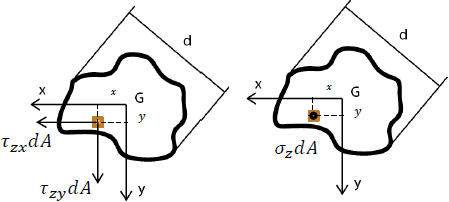
\includegraphics[width=0.5\linewidth]{Immagini_2/screenshot003}
	\label{fig:screenshot003}
\end{figure}

	Adesso, attraverso le equazioni di equilibrio al contorno, si possono legare le tensioni alle deformazioni, le caratteristiche della sollecitazione sulla $S_l$ perciò saranno:
\[\begin{matrix}
	\begin{aligned}
		N = \int_A P_zdA = \int_A \sigma_zdA  \hspace{1cm} & M_x = \int_A P_zydA = \int_A \sigma_zydA  \\
		T_x = \int_A P_xdA = \int_A \tau_{zx}dA \hspace{1cm} &  M_y = -\int_A P_zxdA = -\int_A \sigma_zxdA \\
		T_y = \int_A P_ydA = \int_A \tau_{zy}dA \hspace{1cm} &  M_z = \int_A (\tau_{zy}x -\tau_{zx}y)dA
	\end{aligned}	
\end{matrix}\]
	

	Il problema si riduce così alla determinazione dello stato tensionale a partire dalla conoscenza dell'equilibrio delle caratteristiche della sollecitazione. 

	Sapendo inoltre che le equazioni trovate sono valide per una sezione del materiale, essendo questo LOI per ipotesi, varranno per tutto il materiale. \newline

   \begin{en} [\textbf{Principio di De SaintVenant}]
		Se ad un elemento superficiale di un solido è applicato un sistema di forze autoequilibrato, lo stato di tensione nei punti del solido a sufficiente distanza dall’elemento caricato è praticamente nullo (distanza di estinzione).
	\end{en}  
	
	Ne consegue che, se si applica alla base dell'elemento trave un sistema di forze autoequilibrato, ad una certa distanza da tale base lo stato di tensione non dipende dalla
	distribuzione dei carichi effettivi applicati sulle basi ma soltanto dalle caratteristiche della sollecitazione. \newline	
	
	La distanza a cui l’effetto dei carichi in equilibrio sulle basi diventa nullo è detta distanza di estinzione e risulta in genere pari alla dimensione massima $ d $ della sezione retta.\newline 
	
	Per cui se si determina lo stato tensionale interno per una distribuzione particolare delle sollecitazioni superficiali
	sulle basi allora si è in grado di determinare lo stato tensionale per una qualsiasi distribuzione con le
	stesse caratteristiche. \newline 
	
	Come si scrive il tensore delle tensioni di De Saint Venant? 
	
	Le caratteristiche della sollecitazione varieranno lungo l'asse per cui in ogni punto dell'asse varrà una mappatura di tensioni lungo la sezione. \newline	
	 
	In questo caso sulla base sono presenti 3 tensioni: 
	\begin{equation}
	\boxed{[\sigma] = \left[ \begin{array}{ccc}
		0 & 0 & \tau_{xz} \\
		0 & 0 & \tau_{yz} \\
		\tau_{zx} & \tau_{zy} & \sigma_z
	\end{array}\right]}
	\end{equation} 
	Le soluzioni di questo tensore delle tensioni sono dette soluzioni alla De Saint Venant. \newline 

	Come si comporta la trave di De Saint Venant?
	
	Fisicamente equivale a considerare la trave come un insieme di fibre longitudinali \textit{spaghettiformi} che trasferiscono
	azioni mutue tangenzialmente alla direzione delle fibre stesse.  
	\begin{figure}[H]
		\centering
		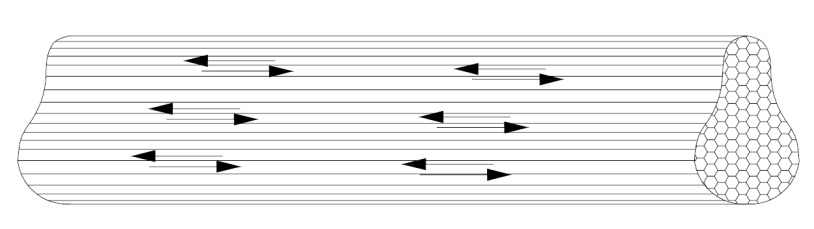
\includegraphics[width=0.5\linewidth]{Immagini_2/screenshot004}
		\label{fig:screenshot004}
	\end{figure}	
	
\begin{itemize}
	\item[$\Rightarrow$] Le equazioni indefinite di equilibrio diventano: 
	\[ \begin{cases}
		\begin{aligned}
			\frac{\partial \tau_{zx}}{\partial z} & =0 \\
			
			\frac{\partial \tau_{zy}}{\partial z} & =0 \\
			
			\frac{\partial \tau_{xz}}{\partial x} + \frac{\partial \tau_{yz}}{\partial y} + \frac{\partial\sigma_z}{\partial z} & =0 \\
		\end{aligned}
	\end{cases}\]
	Dalle prime due equazioni si deriva che il vettore delle tensioni $\vec{\tau}_z=(\tau_{xz},\tau_{yz})$ risulta costante in $ z $ e quindi indipendente da $ z $, ovvero su di un piano ortogonale a $z$ agisce un campo vettoriale del tipo:
	\[ \vec{\tau}_z=\tau_{xz}(x,y)\hat{i} + \tau_{yz}(x,y)\hat{j} \]
	Per ottenere la tensione normale si derivi la terza equazioni in $z$:
	\[\frac{\partial^2 \tau_{xz}}{\partial x\partial z} + \frac{\partial^2 \tau_{yz}}{\partial y\partial z} + \frac{\partial^2\sigma_z}{\partial^2 z}  = 0 \]
	\[ \frac{\partial^2\sigma_z}{\partial^2 z}  = 0 \Rightarrow \frac{\partial\sigma_z}{\partial z}  = cost \]
	\[ \sigma_z (x,y,z)= \dfrac{z}{l}\sigma_z (x,y,z) + \dfrac{l-z}{l}\sigma_z (x,y,z)\]
	$\sigma_z$ è lineare, lungo la fibra varia linearmente. \newline


	\item[$\Rightarrow$] Quello a cui ci si riconduce è uno stato tensionale piano: ridotto il tensore delle tensioni ad un tensore principale, ovvero se delle infinite terne disponibili ci si limita a quelle principali, se i 3 pivot sono non nulli lo stato di tensione è tridimensionale, se uno è nullo lo stato sarà bidimensionale e se due sono nulli lo stato sarà monodimensionale. \newline 

	Le direzioni principali si ricavano dal tensore delle tensioni generico ponendo il determinale pari a zero, nel caso di De Saint Venant: 
	\[ \det[\sigma] \equiv 0 \]
	Esistono allora sicuramente almeno due soluzioni non nulle, il problema sarà così definibile piano.
	
	Poiché lo stato tensionale è piano, il piano delle tensioni sarà individuato dal vettore della tensione tangenziale $\tau$ e dal vettore della tensione normale $\sigma$, da cui ne consegue il fatto che i punti della stessa fibra avranno lo stesso piano delle tensioni: lungo lo spaghetto $\tau_{xz}, \tau_{yz}$ sono costanti, ma non è detto che non possano variare nelle altre direzioni. \newline
	
	Quali sono a questo punto le direzioni principali? Una sarà data da $z$, l'altra da $\tau$ e la terza verrà ricavata di conseguenza. 
\end{itemize}
		
\section{Forza Normale Centrata}
	Si cerchi una soluzione al problema applicando la più semplice delle sollecitazioni, una tensione monodimensionale per cui la risultante delle forze esterne applicate sulle basi estremali sia equivalente ad una forza centrata N:
	\[ \begin{cases}
		p_x =0 \\
		p_y = 0 \\
		p_z = c
	\end{cases} \hspace{1cm} \begin{cases}
	\tau_{xz} = p_x = 0 \\
	\tau_{yz} = p_y = 0 \\
	\sigma_z = p_z = c
\end{cases}\]
	Ne derivano le seguenti caratteristiche della sollecitazione:
	\[\begin{matrix}
		\begin{aligned}
			N = \int_A \sigma_zdA = cA \hspace{1cm} & M_z = \int_A (\tau_{zy}x -\tau_{zx}y)dA = 0 \\
			T_x = \int_A \tau_{zx}dA = 0 \hspace{1cm} & M_x = \int_A \sigma_zydA = c\int_A ydA = cS_x  \\
			T_y = \int_A \tau_{zy}dA = 0 \hspace{1cm} & M_y = -\int_A \sigma_zxdA = -c\int_A zxdA = -cS_y
		\end{aligned}	
	\end{matrix}\]
 	Dove con $S_x, S_y$ si sono identificati i momenti statici, questi nulli se - come per ipotesi - ci si è posti in un sistema di riferimento baricentrale.  (Ricordi la geometria delle aree?) \newline
 	
 	La sollecitazione si configura così essere semplicemente di sforzo normale solo se l’asse $ z $ è baricentrico per la trave.
 	\begin{figure}[H]
 		\centering
 		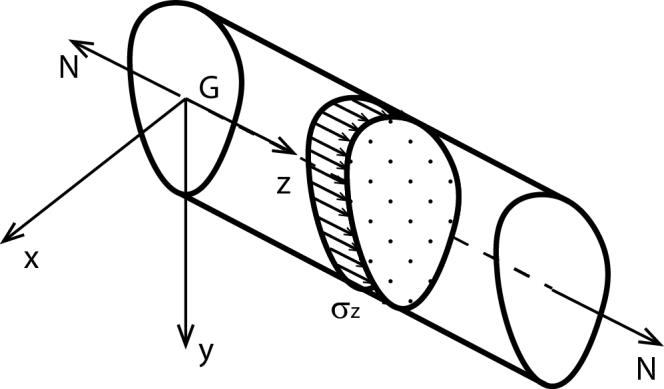
\includegraphics[width=0.5\linewidth]{Immagini_2/screenshot005}
 		\label{fig:screenshot005}
 	\end{figure}	
 	Si integrino le condizioni di equilibrio, in $z$: $\begin{cases}
 		\tau_{zx} = cost \\
 		\tau_{zy} = cost 
 	\end{cases}$ \newline per definizione le tensioni agli estremi sono nulle (è applicata solo N) e dunque \newline $\tau_{zx} = \tau_{zy} = 0 ~ \forall z  \in  (0,l)$ queste, sostituite nella terza equazione di equilibrio portano a:
 \[ \dfrac{\partial\sigma_z}{\partial z} = 0 \Rightarrow \sigma_z = cost ~ \text{in $z$}\] 
 	Poiché in $z=l$ la tensione è nota:
 \[ 	N = \int_A \sigma_zdA = cA \]
	 Ma è noto che: \[ \sigma_z = c\] Allora:  \[N  = \sigma_zA \Rightarrow \sigma_z = \frac{N}{A} \] Verificando la forma del tensore delle tensioni per stato tensionale monoassiale:
 \begin{equation}
 \boxed{	\left[ \begin{array}{ccc}
 	0 & 0 & 0 \\
 	0 & 0 & 0 \\
 	0 & 0 & \dfrac{N}{A}
 \end{array}\right]} 
 \end{equation}
 	Ricordi che la terna principale è una terna di assi per la quale il tensore delle
 	tensioni è una matrice diagonale? In questo caso essendo la matrice diagonale, si conclude che la terna principale sarà così formata dall'asse $z$ e da qualsiasi altri assi che siano ortogonali a $z$ e tra di loro. \newline
\begin{itemize}
	 	
 \item[$\Rightarrow$] Si valutino a questo punto la congruenza ed il legame costituivo, condensati questi nelle relazioni di Navier, integrando queste equazioni si può così risalire agli spostamenti in maniera univoca.
 	\[ 
 \begin{cases}
 	\begin{aligned}
 		\varepsilon_{xx} =   \frac{\partial u_x}{\partial x} = \dfrac{1}{E}[\sigma_x - \nu(\sigma_y + \sigma_z)] = -\dfrac{\nu N}{EA} \\
 		\varepsilon_{yy} =   \frac{\partial u_y}{\partial y} = \dfrac{1}{E}[\sigma_y - \nu(\sigma_x + \sigma_z)] = -\dfrac{\nu N}{EA} \\
 		\varepsilon_{zz} =   \frac{\partial u_z}{\partial z} = \dfrac{1}{E}[\sigma_z - \nu(\sigma_x + \sigma_y)] = \dfrac{ N}{EA} \\
 	\end{aligned}
 \end{cases} \hspace{1cm} \begin{cases}
 	\begin{aligned}
 		\gamma_{xy} =   \frac{\partial u_y}{\partial x} + \frac{\partial u_x}{\partial y} = \dfrac{1}{G} \tau_{xy} = 0\\
 		\gamma_{yz} =   \frac{\partial u_y}{\partial z} + \frac{\partial u_z}{\partial y} = \dfrac{1}{G} \tau_{xz} = 0 \\
 		\gamma_{zx} =   \frac{\partial u_z}{\partial x} + \frac{\partial u_x}{\partial z} = \dfrac{1}{G} \tau_{yz} = 0 \\
 	\end{aligned}
 \end{cases}
 \]
 	Ricordi che $EA$ è il modulo di rigidezza? \newline 
 	
 	 Quali sono i risultati notevoli? Innanzitutto si nota subito che a seguito di una trazione che c'è un allungamento in direzione $z$ dato da $\varepsilon_{zz} = \dfrac{ N}{EA}$ e una diminuzione di sezione (strizione!) lungo $ x $ e lungo $ y $ data dai contributi $\varepsilon_{xx} = \varepsilon_{yy} = -\dfrac{\nu N}{EA}$, si nota infine  la più totale assenza di distorsioni, i termini in $\gamma$ sono tutti nulli, in questo modo la sezione NON si modificherà, non cambiando gli angoli tra le rette/fibre. 
 	
 	\item[$\Rightarrow$] Adesso ci si pone di analizzare gli spostamenti associati a questo tipo di sforzo normale centrato: si integreranno le equazioni di Navier appena scritte.
 \[ \begin{cases}
 	\begin{aligned}
 	u & = -\dfrac{\nu N}{EA}x + u_0(z,y) \\
 	v & = -\dfrac{\nu N}{EA}y + v_0(z,x) \\
 	w & = \dfrac{N}{EA}z + w_0(x,y)
 	\end{aligned}
 \end{cases} \]
	Si ottengono così degli spostamenti definiti a meno di funzioni, se queste funzioni descrivono un moto che non dà contributi in termini direzionali deformativi, il corpo si muoverà nello spazio senza subire ulteriori tensioni e deformazioni compiendo un \textbf{moto rigido} e queste funzioni potranno essere trascurate. 
	
	Si sostituiscano perciò tali funzioni all'interno delle equazioni degli allungamenti e distorsioni:
		\[ 
	\begin{cases}
		\begin{aligned}
			\varepsilon_{0x} =   \frac{\partial u_0}{\partial x} = 0 \\
			\varepsilon_{0y} =   \frac{\partial v_0}{\partial y} = 0 \\
			\varepsilon_{zz} =   \frac{\partial w_0}{\partial z} = 0 \\
		\end{aligned}
	\end{cases} \hspace{1cm} \begin{cases}
		\begin{aligned}
			\gamma_{0xy} =   \frac{\partial u_0}{\partial x} + \frac{\partial u_0}{\partial y} = 0\\
			\gamma_{0yz} =   \frac{\partial v_0}{\partial z} + \frac{\partial w_0}{\partial y} =  0 \\
			\gamma_{0zx} =   \frac{\partial w_0}{\partial x} + \frac{\partial u_0}{\partial z} =  0 \\
		\end{aligned}
	\end{cases}
	\]
	Come ci si poneva di dimostrare a tali funzioni non sono associati nè allungamenti nè distorsioni, perciò sono caratteristiche di un moto rigido. \newline
	
	Gli spostamenti sono così infine definiti a meno di un moto rigido:
	\begin{equation}		 
	\boxed{	\begin{cases}
		\begin{aligned}
			u & = -\dfrac{\nu N}{EA}x  \\
			v & = -\dfrac{\nu N}{EA}y  \\
			w & = \dfrac{N}{EA}z 
		\end{aligned}
	\end{cases}}
	\end{equation}

\end{itemize}
	In conclusione, lo sforzo normale genera una trasformazione omotetica del solido, ovvero una variazione di volume ma non di forma in base al segno di $N$:
	\[ \begin{cases}
		N>0 ~ \text{Trazione, aumento di volume} \\
		N<0 ~ \text{Compressione, diminuzione di volume}
	\end{cases}
	\]
	Rimanendo sempre nel campo di sollecitazioni elastiche,
	per $ N>0 $ il volume aumenta, c'è di mezzo un modulo di Poisson, la trave si allunga di più di quanto si strizioni, le fibre longitudinali si allungano più di quanto non si
	accorcino quelle trasversali: i punti sul mantello si avvicinano al baricentro rendendo tuttavia la configurazione deformata affine a quella indeformata è per questo che la variazione di volume è comunque positiva: l’asse baricentrico viene allungato in direzione $ z $, al contrario delle altre fibre longitudinali che subiscono
	anche una strizione (avvicinamento all’asse baricentrico).
	
	Per la compressione $ N<0 $ invece, la trave si comprime assialmente più di quanto si allunghi lateralmente. \newline
	
	L'entità dello spostamento delle fibre è proporzionale alla quota $xy$: la strizione diviene maggiore allontanandosi dalla zona centrale. \newline
	
	Inoltre la sezione retta resta tale spostandosi su di un piano parallelo cambiando però forma:
	\[ x' = x + u = x \left(1-\dfrac{\nu N}{EA}\right) \hspace{1cm } y' = y + v = y \left(1-\dfrac{\nu N}{EA}\right) \hspace{1cm } z' = z + w = w \left(1-\dfrac{ N}{EA}\right)\]
	
	
\newpage		
\documentclass{article}
\usepackage[left=0.85in, right=0.85in, top=0.5in, bottom=0.95in]{geometry}
\usepackage[T1]{fontenc}
\usepackage[utf8]{inputenc}
\usepackage[italian]{babel}
\usepackage{graphicx}
\usepackage{wrapfig2}
\usepackage{amsmath}
\usepackage{amssymb}
\usepackage{cases}
\usepackage{gensymb} %simboli come ° = \degree  etc etc
\usepackage{subcaption}
\usepackage{hyperref}
\hypersetup{
	colorlinks=true,
	linkcolor=blue,    
	urlcolor=blue,
%	pdfpagemode=FullScreen,
}
\urlstyle{same}
\usepackage{changepage}
\usepackage{lastpage, epstopdf}
\usepackage{fancyhdr}
\usepackage{tcolorbox}
\usepackage{background}
\usepackage{mathtools}
\usepackage{tikz}
\usetikzlibrary{patterns}


%=======HEADER & FOOTER=======%
\def\lesson{Lezione N 3}
\def\outcome{\textbf{Learning Outcomes:} Outcomes go here. }

\pagestyle{fancy}
\fancyhf{}
\renewcommand{\headrulewidth}{0pt}
\renewcommand{\footrulewidth}{1.4pt}
\lfoot{A.M. $\diamond$ \the\year}
\cfoot{\thepage}
\rfoot{\lesson}

%=======CORNELL STYLE FORMAT=======%
\SetBgScale{1}
\SetBgAngle{0}
\SetBgColor{black}
\SetBgContents{\rule{1pt}{0.85\paperheight}}
\SetBgHshift{-1.6in}
\SetBgVshift{-0.1in}

%=======CUSTOM BOXES=======%

\parindent 0ex

%=======BODY=======%
\begin{document}
	\setcounterpageref{secnumdepth}{0}
	\section*{Parte 3} %Date: \hrulefill}
%	\begin{tcolorbox}{\outcome}\end{tcolorbox}

\begin{adjustwidth}{2in}{} 
	
\textbf{{\Large De Saint Venant: Flessione Retta}} \mbox{} \newline
		Si voglia studiare una sollecitazione associata tale che su una faccia la risultante  sia un momento e sull'altra lo stesso momento uguale e opposto: imponendo così una flessione uniforme genero un momento flettente costante su tutta la trave in modo che le fibre trazionate si troveranno in basso e quelle compresse in alto. 
		
\begin{figure}[H]
	\centering
	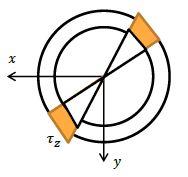
\includegraphics[width=0.5\linewidth]{Immagini/screenshot001}
	\label{fig:screenshot001}
\end{figure}


		Il momento $M_x$ sulla faccia estremale si ottiene così attraverso una determinata distribuzione di pressione, che ipotizzo lungo $z$ essere lineare in $ x $ ed $ y $. 
		
		\[\begin{cases}
			p_x = 0 \\
			p_y = 0 \\
			p_z = a + bx + cy\end{cases} \Rightarrow \begin{cases}
			\tau_{zx} = p_x = 0 \\
			\tau_{zy} = p_y = 0 \\
			\sigma_z = p_z =  a + bx + cy  \\
		\end{cases}  \] 

		Le caratteristiche della sollecitazione sulla $S_l$ saranno:
		\[\begin{matrix}
			\begin{aligned}
				N = \int_A \sigma_zdA = aA + bS_y + cS_x  \hspace{1cm} & M_z = \int_A (\tau_{zy}x -\tau_{zx}y)dA = 0 \\
				T_x = \int_A \tau_{zx}dA = 0 \hspace{1cm} & M_x = \int_A \sigma_zydA = aS_x + bI_{xy} + cI_X \\
				T_y = \int_A \tau_{zy}dA = 0 \hspace{1cm} & M_y = -\int_A \sigma_zxdA = -aS_y - bI_y - cI_{xy}
			\end{aligned}	
		\end{matrix}\]
		Con $S_i$ momento statico, $I_i$ momento d'inerzia, $I_{xy}$ momento centrifugo.
		
		Ottengo in questo modo 3 sollecitazioni distinte ognuna dipendente in modo indipendente dalle altre attraverso un coefficiente di $\sigma_z$. \newline 
		
		Cambiando riferimento in uno baricentrico con assi principali d'inerzia, ottengo l'annullamento di tutti i momenti centrifughi e statici, riconducendomi a sole tre equazioni:
		\[ N = aA \hspace{1cm} M_x = cI_X \hspace{1cm} M_y = - bI_y  \]
		Per avere soltanto sollecitazione flessionale retta e solo un momento lungo la $x$, è necessario annullare i contributi $a$ e $b$, in questo modo, ipotizzando una distribuzione di pressione dipendente solo da $y$ e lineare con essa, si ottiene che: 
		\[\sigma_z = cy\]
		E dunque: 
		\[ N = 0 \hspace{1cm} M_x = cI_X \hspace{1cm} M_y = 0  \]
		L'ipotesi di De Saint Venant per avere flessione retta è quella per cui la distribuzione di tensione ha un andamento lineare lungo la $y$. \newline 
		
		Risolto l'equilibrio esterno si passi ora all'equilibrio interno:
			\[ \begin{cases}
			\begin{aligned}
				\frac{\partial \tau_{zx}}{\partial z} & =0 \\
				
				\frac{\partial \tau_{zy}}{\partial z} & =0 \\
				
				\frac{\partial \tau_{xz}}{\partial x} + \frac{\partial \tau_{yz}}{\partial y} + \frac{\partial\sigma_z}{\partial z} & =0 \\
			\end{aligned}
		\end{cases}\]
		Integrando in $z$ le prime due si ottiene:
		\[\begin{cases}
			\tau_{zx} = cost \\
			\tau_{zy} = cost 
		\end{cases}\]
		All'esterno la pressione indotta non introduce alcuna presenza di tensioni tangenziali, per questo motivo, le tensioni tangenziali oltre che essere costanti, sono anche nulle lungo z. 
		
		Tale risultato, sostituito nella terza equazione, porta a:
		\[ \frac{\partial\sigma_z}{\partial z}  =0\]
		Concludendo che la tensione $\sigma_z$ è costante lungo z. \newline 
		
		Poiché la tensione è nota in $z = l$ ed è quella imposta secondo:
		\[M_x = cI_X \Rightarrow c = \dfrac{M_x}{I_x} \]
		E dalla conoscenza che:
		\[ \sigma_z = cy\]
		Si conclude che: 
		\[ \sigma_z = \dfrac{M_x}{I_x}y \]
		Anche in questo caso, come per lo sforzo normale, ci si riconduce ad uno stato tensionale monoassiale: 
		\[ \left[\begin{array}{ccc}
			0 & 0 & 0 \\
			0 & 0 & 0 \\
			0 & 0 & \dfrac{M_x}{I_x}y
		\end{array}\right]\]
		Ma con la sostanziale differenza che questo è lineare.
		
		Per lo sforzo normale avevo una tensione uniforme sulla sezione e uguale per tutte le sezioni; qui l'andamento rimane sì il medesimo per tutte le sezioni, ma sulla singola sezione la $\sigma_z$ varia sulle $y$ a farfalla, è quindi linearmente dipendente dalla quota $y$, dalla distanza del punto generico $P$ della sezione e dall'asse dei momenti, l'asse rispetto al quale applico il momento flettente, d'altronde per valutare il momento $M_x$ la distanza che si dovrà prendere in considerazione è la $y$. 
		
		Tutti i punti della sezione con la medesima quota $ y $ avranno perciò la stessa tensione $\sigma_z$. 
\newpage		
		La terna principale sarà anche in questo caso formata da $ z $ e due qualsiasi assi
		appartenenti al piano ortogonale a $ z $ e tra loro ortogonali.
		
\begin{figure}[H]
	\centering
	\includegraphics[width=0.5\linewidth]{Immagini/screenshot002}
	\label{fig:screenshot002}
\end{figure}

		Il luogo dei punti caratterizzato da $y=0$ sulla sezione è detto linea o asse neutro delle tensioni, su tutti quei punti la tensioni che agisce è nulla. Tutte queste linee, messe in successione, descrivono un piano, il piano neutro della trave, il luogo dei punti del volume caratterizzato da tensione nulla, completamente scarico. 
		
		In questo caso l'asse neutro coincide con quello baricentrale. \newline
		
		Nel caso di flessione retta, ovvero di quella flessione generata da un momento flettente applicato lungo un asse principale di inerzia, l'asse neutro coincide con l'asse dei momenti. \newline 
		
		Si chiama asse delle sollecitazioni quello perpendicolare a quello dei momenti.
		
		Nel caso di flessione retta, l'asse delle sollecitazioni è perpendicolare all'asse neutro che coincide con quello dei momenti e quello baricentrico. \newline
		
		Al contrario, esistono punti dove la tensione è massima, questi sono altresì caratterizzati dalla massima distanza dall'asse baricentrico $x$; in termini di modulo, sarà il punto più lontano da tale asse ad essere il più sollecitato, a trazione o compressione. \newline
		
		\item[!!] È importante notare che un grafico a farfalla siffatto NON è la reale rappresentazione del momento su $z$, questo uscente/ortogonale dal piano del foglio/sezione, ma riporta soltanto L'ANDAMENTO del modulo del vettore $|\sigma_z|$. 
		
		\item[!!] A seguito di un $M_x$ positivo, si viene a formare sulla sezione una parte di trave sollecitata a ~ $  \underset{+}{trazione} $ e un'altra sollecitata a ~ $ \underset{-}{compressione} $.

		Alla massima distanza tra un massimo ed un minimo avrò, in termini di modulo, il momento massimo. 

		Tra le infinite soluzioni equilibrate, l’unica
		congruente sarà data dalla risoluzione delle seguenti equazioni di Navier:
			\[ 
		\begin{cases}
			\begin{aligned}
				\varepsilon_{xx} =   \frac{\partial u_x}{\partial x} = \dfrac{1}{E}[\sigma_x - \nu(\sigma_y + \sigma_z)] = -\dfrac{\nu M_x}{EI_x}y \\
				\varepsilon_{yy} =   \frac{\partial u_y}{\partial y} = \dfrac{1}{E}[\sigma_y - \nu(\sigma_x + \sigma_z)] = -\dfrac{\nu M_x}{EI_x}y \\
				\varepsilon_{zz} =   \frac{\partial u_z}{\partial z} = \dfrac{1}{E}[\sigma_z - \nu(\sigma_x + \sigma_y)] = \dfrac{M_x}{EI_x}y\\
			\end{aligned}
		\end{cases} \hspace{1cm} \begin{cases}
			\begin{aligned}
				\gamma_{xy} =   \frac{\partial u_y}{\partial x} + \frac{\partial u_x}{\partial y} = \dfrac{1}{G} \tau_{xy} = 0\\
				\gamma_{yz} =   \frac{\partial u_y}{\partial z} + \frac{\partial u_z}{\partial y} = \dfrac{1}{G} \tau_{xz} = 0 \\
				\gamma_{zx} =   \frac{\partial u_z}{\partial x} + \frac{\partial u_x}{\partial z} = \dfrac{1}{G} \tau_{yz} = 0 \\
			\end{aligned}
		\end{cases}
		\]
		Ecco il risultato: l'allungamento su $z$ è quello responsabile delle fibre tese e compresse in \textit{meccanica dei solidi}: tanto è maggiore l'allungamento quanto sarà maggiore la distanza $y$.
		\[\begin{cases}
			y>0 ~ \text{allungamento} \\
			y<0 ~\text{accorciamento}
		\end{cases}\]

\begin{figure}
	\centering
	\begin{tikzpicture} [>=latex]
		%\draw [help lines] (0,0) grid (6,6);
		\draw[thick] (0,0) rectangle (4, 2);
		\draw[thick, green] (-1,0.25) -- (1,2) -- (3,2) -- (5, 0.25);
		\draw[thick, green] (5,0.25) arc (0:-180:3 and 0.5);
		\draw[ ->, thick] (5.5,0.25) arc (0:45:0.5 and 2);
		\draw[ ->, thick] (-1.5,0.25) arc (180:135:0.5 and 2);		
	\end{tikzpicture}
\end{figure}
		
		Integrando le relazioni così ottenute da Navier ottengo gli spostamenti, questi sono definiti a meno di 3 funzioni di integrazione che non posso ignorare a priori a meno che non descrivano un moto rigido, infatti questo per definizione non concorrerà allo stato tensionale e deformativo della trave.
		\[ \begin{cases}
			\begin{aligned}
				u & = -\dfrac{\nu M_x}{EI_x}yx + u_0(z,y) \\
				v & = -\dfrac{1}{2}\dfrac{\nu M_x}{EI_x}y^2 + v_0(z,x) \\
				w & = \dfrac{M_x}{EI_x}yz + w_0(x,y)
			\end{aligned}
		\end{cases} \]
		Sostituisco le $ u_0,  v_0,  w_0$ incognite nella formulazione dello scorrimento $xt$, e in questo caso differentemente dallo sforzo normale, si ottiene:
		\[ 	\gamma_{xy} =   \frac{\partial u}{\partial y} + \dfrac{\partial v}{\partial x} = -\dfrac{\nu M_x}{EI_x}x + \dfrac{\partial u_0(z,y)}{\partial y} + dfrac{\partial v_0(z,x)}{\partial x} = 0\] 
		Derivando rispetto ad $x$:
		\[  \dfrac{\partial^2 v_0(z,x)}{\partial x^2} = \dfrac{\nu M_x}{EI_x}  \]
		Integrando due volte rispetto ad $x$:
		\[  v_0 = \dfrac{1}{2}\dfrac{\nu M_x}{EI_x}x^2 + \underbrace{xv'_0(z) + v'_1(z)}_\text{$v_1(x,z)$} \]
		E quindi si giunge a: 
		\[ \begin{cases}
			\begin{aligned}
				u & = -\dfrac{\nu M_x}{EI_x}yx + u_0(z,y) \\
				v & = \dfrac{1}{2}\dfrac{\nu M_x}{EI_x}(x^2 - y^2) + v_1(x,z) \\
				w & = \dfrac{M_x}{EI_x}yz + w_0(x,y)
			\end{aligned}
		\end{cases} \]
		La nuova terna di spostamenti però non descrive ancora un moto rigido:
		\[\gamma_{yz} =   \frac{\partial v}{\partial z} + \frac{\partial w}{\partial y} = \dfrac{\partial v_1(x,z)}{\partial z} + \dfrac{M_x}{EI_x}z +\dfrac{\partial w_0(x,y)}{\partial y} = 0\]
		Similmente a poco sopra derivo rispetto a $z$ ed integro due volte rispetto a $z$: 
		\[  \dfrac{\partial^2 v_1(x,z)}{\partial z^2} = - \dfrac{M_x}{EI_x}  \]
		\[  v_1 = -\dfrac{1}{2}\dfrac{M_x}{EI_x}z^2 + v_2(x,z) \]
		Ora le funzioni $ u_0,  v_2,  w_0$ descrivono un moto rigido: le deformazioni ad esse associate sono nulle:
		\[\begin{cases}
			\begin{aligned}
				\gamma_{xy} =   \frac{\partial v}{\partial x} + \frac{\partial u}{\partial y} = \dfrac{\nu M_x}{EI_x}x - \dfrac{\nu M_x}{EI_x}x  = 0\\
				\gamma_{yz} =   \frac{\partial v}{\partial z} + \frac{\partial w}{\partial y} = + \dfrac{M_x}{EI_x}z + \dfrac{M_x}{EI_x}z = 0 \\
				\gamma_{zx} =   \frac{\partial u_z}{\partial x} + \frac{\partial u_x}{\partial z} = 0 \\
			\end{aligned}\end{cases}\]
		
		 E quindi le rispettive funzioni sono eliminabili dalla soluzione finale, che in questo modo sarà:
		\[\boxed{\begin{dcases}			
				u & = -\dfrac{\nu M_x}{EI_x}yx + u_0(z,y) \\
				v & = -\dfrac{1}{2}\dfrac{\nu M_x}{EI_x}(x^2 - y^2)  -\dfrac{1}{2}\dfrac{ M_x}{EI_x}z^2 \\
				w & = \dfrac{M_x}{EI_x}yz + w_0(x,y)	
		\end{dcases}} \]
		
		La linea d'asse (l'asse baricentrico) si trova sostituendo $x=y=0$, lo spostamento ad essa associato è:
		\[ v  = -\dfrac{1}{2}\dfrac{ M_x}{EI_x}z^2 \] 
		Quadratico rispetto a $z$, il che significa che la linea d'asse non subisce spostamenti $u$ sul piano della sezione e quindi lungo l'asse dei momenti; non subisce neanche allungamenti $w$, ma subisce solamente degli spostamenti $v$ ortogonali al sua asse e a quello dei momenti. \newline 
		
		Se si rappresenta la trave in un piano $xy$, la linea d'asse, a seguito di un momento $M_x$ si inflette nel modo seguente, subendo solo spostamenti in direzione $y$:
		
\begin{figure}[H]
	\centering
	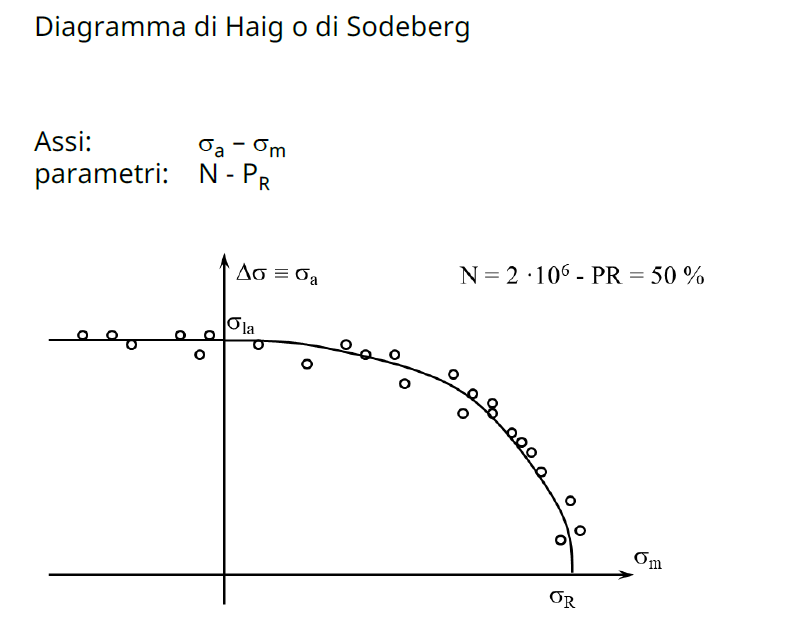
\includegraphics[width=0.5\linewidth]{Immagini/screenshot003}
	\label{fig:screenshot003}
\end{figure}

		La linea d'asse rimane perciò in un piano chiamato piano di inflessione, ortogonale questo all'asse dei momenti, in questo caso $yz$. \newline 
		
		Si valuti adesso rotazione e curvatura dell'andamento quadratico. 
		\[ \chi = \dfrac{1}{R} = \dfrac{\ddot{v}}{(1+\dot{v}^2)^{3/2}}\]
		Dove $v$ è l'abbassamento. Inoltre, sotto le ipotesi di piccoli spostamenti e di Bernoulli, per la quale le sezioni rette continuano ad essere rette per ogni sollecitazione applicata $\dot{v}\approx 0$ e dunque: 
		\[ \chi = \dfrac{1}{R} = \ddot{v} = \dfrac{ M_x}{EI_x} \]
		Essendo la curvatura costante in $z$, la deformata d'asse sarà a curvatura costante, inoltre, come non notare che la curvatura dipende dal momento stesso $M_x$ e dal modulo di rigidezze flessionale $EI_x$? Tanto maggiore sarà quest'ultimo, infatti, tanto maggiore sarà il raggio di curvatura e tanto minore sarà la curvatura: Maggiore sarà $EI_x$ minore sarà la deformabilità della trave a flessione. \newline 
		
		A parità di momento flettente, per avere piccole deformate flessionali o scelgo un materiale più rigido o scelgo una sezione maggiore, la sezione della trave è d'altro canto legata al momento d'inerzia, che ad esempio, per trave a sezione quadrata:
		\[ I= \dfrac{bh^3 }{12}\]
		Con $b,h$ dimensioni della sezione. \newline 
		
		Ma se fossi in grado di realizzare la stessa inerzia on meno materiale? Sarebbe auspicabile, meno peso, meno ingombro e meno costo \dots 
		
		Dalla definizione, il momento d'inerzia vale: 
		\[  I_x = \int_A y^2dA\]
		Infatti questo non dipende da come è distribuito il materiale rispetto all'asse $x$ ma solo da com'è distribuito intorno all'asse $y$. 
		
		Se la stessa quantità di materiale  si riesce a distribuire il più lontano possibile dall'asse $ x $ e quindi a maggiori quote $y$, ottengo di fatto un maggiore momento d'inerzia. 
		
\begin{figure}
	\centering
	\begin{tikzpicture} [>=latex]
		%\draw [thin, help lines] (0,0) grid (10,10);
		\draw[thick] (0,0) rectangle (4, 1);
		\draw[thick] (1.5,1) rectangle (2.5, 4);
		\draw[thick] (0,4) rectangle (4, 5);
		\draw[pattern=north east lines, thick] (0,1) rectangle (1.5, 4);
		\draw[pattern=north east lines, thick] (2.5,1) rectangle (4, 4);
		\draw[->>, thick, red] (2, 5) -- (2, -1) node [pos=1, below] {$M_y$};
		\draw[->, thick] (-0.5, 2.5) -- (4.5, 2.5) node [pos=1, right] {$z$};
		\draw[->, thick] (-0.5, 2.5) -- (-0.5, 1) node [pos=1, below] {$y$};
		\draw[->, thick] (-0.5, 2.5) -- (-2, 1.5) node [pos=1, below] {$z$};
		\draw[->>, thick, blue] (-0.5, 2.5) -- (-2, 2.5) node [pos=1, left] {$M_x$};
	\end{tikzpicture}
\end{figure}

		\item[!!] Le stessa sezione però, sollecitata secondo l'asse di un momento $M_y$ non potrebbe comportarsi allo stesso modo, infatti in questo caso è importante  che dipenderà questo dalla distanza a cui è collocato il materiale lungo $x$, in questo  lungo $x$ c'è molta distribuzione di materiale il che comporterà $I_y$ avere un ODG inferiore, ma in cosa si traduce un ODG inferiore sul momento d'inerzia? Ad un ODG superiore sulle tensioni! \newline 
		
		Ritornano alla linea d'asse, si è più che dimostrato come questa non subisca deformazioni ma solo spostamenti: quando applico un'inflessione alla linea d'asse questa per ogni punto in configurazione deformata deve avere la stessa quota $z$ d'altronde vale $w=0$, le sezioni si trovano perciò alla stessa quota $z$ senza allungamenti; la linea d'asse però inflettendosi ha fatto però un percorso ben più lungo perché per arrivare alla stessa quota con una traiettoria curva si vuole un cammino maggiore, mi aspetto allora un allungamento $\varepsilon_{zz}$ che però non c'è, sostituisco allora l'equazione dell'asse baricentrico nello spostamento $w$, ma questo continua ad essere nullo. \newline 
		
		Tale paradosso è giustificato dai piccoli spostamenti, infatti posso scrivere lo spostamento che compie l'asse come somma in quadratura:
		\[ ds^2 \approx dz^2 + dv^2 = dz^2 + \left[\dfrac{M_x}{EI_x}zdz\right]^2 = dz^2 \left[1+ \left(\dfrac{M_xz}{EI_x}\right)^2\right] \]
		Per piccoli spostamenti, che sono quelli con cui lavoriamo:
		\[\left(\dfrac{M_xz}{EI_x}\right)^2 << 1\]
		E quindi si può trascurare:
		\[  ds^2 \approx dz^2 \]
		Nell’ipotesi di piccole deformazioni la lunghezza dell’asse può essere considerata costante. \newline
		
		All'infuori della linea d'asse le fibre si allungano, ciò che si ottiene è perciò una funzione di allungamento/spostamento su $z$ che dipende da $y$:
		\[ z' = z + w = z + \dfrac{M_x}{EI_x}yz = K \left(1-\dfrac{y}{R}\right)\]
		Tanto più ci si sposta lungo la $y$ tanto più le fibre si allungano. 
		
		La sezione subisce così degli spostamenti $w$ proporzionali alla quota $y$, tale spostamento non fa nient'altro che generare una rotazione rigida della sezione che ruoterà a seguito della flessione intorno all'asse dei momenti, dalla definizione la rotazione è data da: 
		\[  \varphi = -\dfrac{ \partial v}{ \partial z}\]
		
\begin{figure}[H]
	\centering
	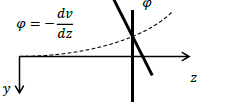
\includegraphics[width=0.5\linewidth]{Immagini/screenshot004}
	\label{fig:screenshot004}
\end{figure}


		Una sezione retta che giace su un piano ortogonale alla linea d’asse, una volta deformata
		continua a giacere su un piano che è ruotato ma che è ancora ortogonale alla linea d’asse (ora
		deformata) e dunque: 
		\[ \varphi(z) = \dfrac{M_x}{EI_x}z \]
		Oppure, equivalentemente, se si considera che lo spostamento $z'$ porta la sezione su un piano ortogonale al piano contenente la deformata della linea d’asse
		la cui traccia sul piano $ yz $ è una retta che passa per il centro del raggio osculatore:
		\[ d\varphi(z) = \dfrac{1}{|R|}ds = \dfrac{M_x}{EI_x}dz \]
		
		All'estremo della trave si ottengono gli stessi valori incontrati in \textit{meccanica dei solidi} della trave a mensola sollecitata con un momento:
		\[ v(l) = -\dfrac{1}{2}\dfrac{M_x}{EI_x}l^2 \hspace{1cm} \varphi(l) = \dfrac{M_x}{EI_x}l\]
		
		Cosa accade ora nella sezione della trave a seguito della flessione? 
		
		A seguito della deformazione associata alla flessione i segmenti rettilinei e paralleli ad $x$ si trasformano in archi di circonferenza il: segmento si inflette secondo una curvatura che abbiamo imparato a riconoscere costante, ottenendo la seguente mappatura della sezione.
		
\begin{figure}[H]
	\centering
	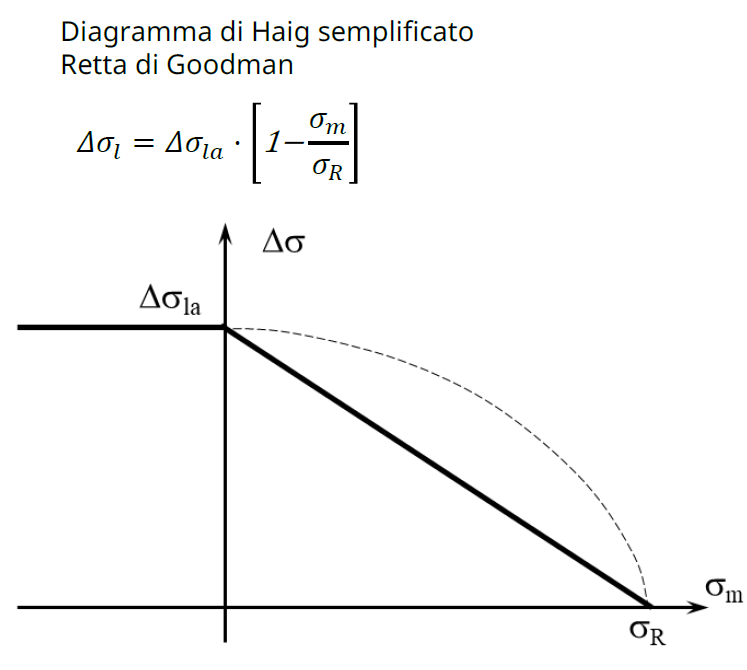
\includegraphics[width=0.5\linewidth]{Immagini/screenshot005}
	\label{fig:screenshot005}
\end{figure}

		La sezione resta piana ma varia la sua forma: ricordando che per le $y>0$ la tensione è di trazione, cosa accade alle fibre della trave? Quelle che si allungano assialmente si avvicinano tra loro, quelle che si comprimono si allontanano tra loro: questo è un meccanismo del materiale per compensare la variazione di volume, le fibre trazionate si avvicinano tra loro occupando meno volume mentre quelle compresse accorciandosi si allontanano tra di loro per occupare più volume.
		
		D'altro canto in una sollecitazione flessionale la deformazione è associata ad una variazione di volume nulla, a differenza della trazione dove caratterizzata da strizione e dunque da una diminuzione di volume. \newline 
		
		In condizioni statiche si ha il bisogno di rispondere principalmente a due domande: 
		\begin{enumerate}
			\item l'oggetto resiste? La tensione che si instaura a seguito delle azioni esterne è minore di quella massima che il materiale può sopportare?
			\item l'oggetto continua a funzionare? È garantita la funzionalità?
		\end{enumerate}
		Se la seconda domanda si traduce nei termini di freccia massima contenuta entro un certo dato da una normativa, alla prima domanda è più articolato rispondere perché implica un confronto tra scalari:
		\[ |\sigma(P)|\leq \sigma_{amm}\]
		Devo quindi tradurre il tensore delle tensioni in una tensione equivalente monodimensionale $\sigma(P)$, e non sempre è immediato. 
		\[\sigma_{amm} = \dfrac{\sigma_{lim}}{X}\]
		Invece tiene conto del fatto che per dimensionare un oggetto che lavorerà in un campo applicativo reale l'effettiva resistenza del materiale sarà ben diversa da quelle studiate in condizioni simil-ideali di laboratorio, è ovvio che si lavorerà con una tensione più bassa data da un opportuno coefficiente di sicurezza normato. È logico poi che in condizioni di operatività può subire delle modifiche, sarà dunque necessario programmare manutenzioni e rilievi per constatare che le opportune e reali condizioni di carico rientrino nelle tensioni ammissibili (e quindi quelle limite ridotte) calcolate in fase di progetto. \newline 
		
		In più, poiché nelle applicazioni strutturali/meccaniche è sempre bene lavorare in campo elastico e non in campo plastico, la tensione limite di cui si dovrà tenere conto in fase di progetto sarà quella di snervamento. \newline 
		
		Ritornando alla definizione del $ \sigma(P) $, nei casi analizzati di sforzo normale e di flessione retta siano in condizioni auspicabili perché entrambe contribuiscono con uno sforzo monodimensionale, è facile dimostrare quindi che per lo sforzo normale in fase di progettazione non sarà tanto importante la forma, ma la sezione dell'oggetto: 
		\[ \sigma_z = \dfrac{N}{A} \leq \sigma_{amm} \Rightarrow A \geq \dfrac{N}{\sigma_{amm}}\]
		Per la flessione retta invece dovrà sussistere la relazione: 
		\[ \sigma_z = \dfrac{M_x}{I_x}y \leq \sigma_{amm} \]
		Noto l'andamento della tensione so che: punti alla stessa quota $y$ hanno tutti lo stesso valore di tensione; ogni sezione presenta esattamente lo stesso andamento; i punti maggiormente sollecitati saranno quelli a massima/minima distanza $y$, tutto ciò porta così ad effettuare due verifiche in dipendenza del materiale utilizzato. 
		
\begin{figure}[H]
	\centering
	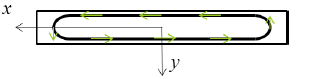
\includegraphics[width=0.5\linewidth]{Immagini/screenshot006}
	\label{fig:screenshot006}
\end{figure}
		
		Il materiale è isotropo e si comporta a trazione e compressione nello stesso modo (ex acciaio)? Utilizzerò allora tra i due il massimo del valore assoluto dei due punti maggiormente sollecitati:
		\[ \sigma_z(P_1) = \dfrac{M_x}{I_x/h_1} \hspace{1cm} \sigma_z(P_2) = \dfrac{M_x}{I_x/h_2}\]
		\[ \max{|\sigma_z(P_1)|; |\sigma_z(P_2)|}\]
		
		Il materiale si comporta in maniera diversa a trazione e compressione (ex ghisa, ceramica, calcestruzzo)? Utilizzerò dei valori specifici ottenuti a trazione o compressione, a seconda di come il materiale lavorerà. \newline 
		
		Ciò che poi in fase di progettazione andrà massimizzato sarà proprio il denominatore di siffatta tensione, condensato nel modulo di resistenza a flessione:
		\[w_x = \dfrac{I_x}{y}\]
		È il rapporto tra l'inerzia e la quota massima di distanza dall'asse baricentrico, e per questo che in fase di progetto è necessario scegliere una sezione che massimizzi l'inerzia e ponga il più lontano possibile dall'asse $x$ il materiale, in questo modo sarà maggiore l'inerzia sull'asse $ x $ e minore la tensione sulla trave.
		
	\newpage
	{\Large \textbf{NOTE}}
%	\vfill
%\begin{tcolorbox}[height=4.5cm]
%	This box has a height of 4.5cm.
%\end{tcolorbox}

%DA DECOMMENTARE PER AVERE LA VERSIONE STAMPABILE A DUE PAGINE 	
%	\newpage
%		\null
%		\vfill
%\begin{tcolorbox}[height=4.5cm]
%	This box has a height of 4.5cm.
%\end{tcolorbox}
%		
\end{adjustwidth}
\end{document}			
\documentclass{article}
\usepackage[left=0.85in, right=0.85in, top=0.5in, bottom=0.95in]{geometry}
\usepackage[T1]{fontenc}
\usepackage[utf8]{inputenc}
\usepackage[italian]{babel}
\usepackage{graphicx}
\usepackage{wrapfig2}
\usepackage{amsmath}
\usepackage{amssymb}
\usepackage{cases}
\usepackage{gensymb} %simboli come ° = \degree  etc etc
\usepackage{subcaption}
\usepackage{hyperref}
\hypersetup{
	colorlinks=true,
	linkcolor=blue,    
	urlcolor=blue,
	pdfpagemode=FullScreen,
}
\urlstyle{same}
\usepackage{changepage}
\usepackage{lastpage, epstopdf}
\usepackage{fancyhdr}
\usepackage{tcolorbox}
\usepackage{background}
\usepackage{tikz}
\usetikzlibrary{patterns}


%=======HEADER & FOOTER=======%
\def\lesson{Lezione N. 4}
\def\outcome{\textbf{Learning Outcomes:} Outcomes go here. }

\pagestyle{fancy}
\fancyhf{}
\renewcommand{\headrulewidth}{0pt}
\renewcommand{\footrulewidth}{1.4pt}
\lfoot{A.M. $\diamond$ \the\year}
\cfoot{Page \thepage}
\rfoot{\lesson}

%=======CORNELL STYLE FORMAT=======%
\SetBgScale{1}
\SetBgAngle{0}
\SetBgColor{black}
\SetBgContents{\rule{1pt}{0.85\paperheight}}
\SetBgHshift{-1.6in}
\SetBgVshift{-0.1in}

%=======CUSTOM BOXES=======%

\parindent 0ex

%=======BODY=======%
\begin{document}
	\setcounterpageref{secnumdepth}{0}
	\section*{Parte 4} %Date: \hrulefill}
%	\begin{tcolorbox}{\outcome}\end{tcolorbox}

\begin{adjustwidth}{2in}{} 
	
\textbf{{\Large De Saint Venant: Flessione Deviata}} \mbox{} \newline
		Si consideri ora l’azione di un momento $ M $ che giace sul piano di
		sezione $ xy $ applicato sulla faccia finale della trave. Si consideri
		il sistema di riferimento $ xyz $ sempre principale di inerzia e baricentrico. Ora il momento è generico e non più coincidente con quello in $x$ o in $y$. 
		
		Si individuano gli assi $m$ asse dei momenti, perpendicolare per definizione all'asse delle sollecitazione $s$, questo è la traccia sulla sezione del piano dove avviene la la rotazione deviata a causa del momento, contiene il piano di rotazione imposto da $M$. \newline 
		
		Una flessione deviata si può studiare attraverso la composizione di flessioni rette applicate secondo gli assi principali di inerzia.
		
\begin{figure}[H]
	\centering
	\label{fig:screenshot001}
	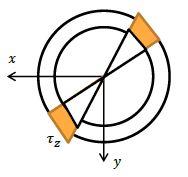
\includegraphics[width=0.5\linewidth]{immagini/screenshot001}
\end{figure}

		In questo modo la sollecitazione è null'altro he una composizione di contributi: 
		\begin{equation} \label{eq:1}
			\sigma_z = \dfrac{M_x}{I_x}y - \dfrac{M_y}{I_y}x
		\end{equation}
		Con segni in accordo al senso di rotazione (antiorario od orario) imposto dal momento. \newline 
		
		Per definizione la traccia sulla sezione del piano neutro è l'asse neutro e si trova attraverso lo studio dei punti non sollecitati:
		\[ \begin{aligned}
			\sigma_z &= 0 \\
			\dfrac{M_x}{I_x}y &- \dfrac{M_y}{I_y}x =0
		\end{aligned} \]
				
\begin{figure}[H]
	\centering
	\label{fig:screenshot002}
	\includegraphics[width=0.5\linewidth]{immagini/screenshot002}
\end{figure}
		
		Si identificano gli angoli $\gamma$, formato dall'asse dei momenti $m$ e dall'asse $x$, e $\beta$ formato dall'asse neutro $n$ e dall'asse $x$.
		\[\dfrac{M_x}{I_x}y - \dfrac{M_y}{I_y}x = 0 \hspace{1cm} \begin{cases}
			M_x = M\cos\gamma \\
			M_y = M\sin\gamma
		\end{cases}\]
		\[\dfrac{ M\cos\gamma}{I_x}y - \dfrac{M\sin\gamma}{I_y}x =0 \Leftrightarrow y = \tan\gamma \dfrac{I_x}{I_y}x\]
		Se, come in questo caso, l'equazione dell'asse neutro non ha il termine noto, passa per l'origine, se il nostro origine è il baricentro, allora l'asse sarà baricentrico.\newline 
		
		L'asse neutro è baricentrico e la sua inclinazione è funzione di $\gamma, I_x, I_y$, ovvero della direzione di applicazione del momento a dalle specifiche caratteristiche della sezione, queste indipendenti dall'entità del momento applicato, in più $M$, l-intensità del momento flettente, non compare: l'asse neutro, oltre che essere baricentrico, è indipendente dal momento applicato. \newline
		Se:
		\[ \tan\beta = \tan\gamma \dfrac{I_x}{I_y} \]
		\[ y = x\tan\beta \]
		
		Si distinguano due casistiche:
		\begin{itemize}
			\item[$ I. $] Se $I_y = I_y \Rightarrow \tan\gamma = \tan\beta $ e l'asse neutro coincide con l'asse dei momenti, ci troviamo nel caso di flessione retta ruotata per sezioni circolari o sezioni caratterizzate da doppio asse di simmetria con distribuzione identica. L’uguaglianza tra
			le inerzie significa che ogni
			riferimento è centrale di inerzia.
			
			\item[$ II. $] Se $I_y \neq I_y \Rightarrow \tan\gamma \neq \tan\beta $ e l'asse neutro NON coincide più con l'asse dei momenti, ci troviamo nel caso di flessione deviata e l'asse delle sollecitazioni non è più ortogonale all'asse neutro ma è inclinato di un angolo $\gamma$.
		\end{itemize}
		 
		
		Perché tutta questa importanza è legata agli assi? Perché sono le tracce dei rispettivi piano. \newline 
		
		Se $\alpha$ identifica l'angolo tra l'asse delle sollecitazioni $s$ e l'asse $x$:
		\[ \alpha = \dfrac{\pi}{2} + \gamma\]
		E l'asse delle sollecitazioni $s$ può essere messo finalmente in relazione con l'asse neutro $n$: 
		\[ \tan\alpha = -\cot\gamma \Rightarrow \tan\gamma = - \dfrac{1}{\tan\alpha}\]
		Poi, ricordando che: 
		\[ \tan\beta = \tan\gamma \dfrac{I_x}{I_y} = - \dfrac{1}{\tan\alpha} \dfrac{I_x}{I_y}\]
		Si giunge infine:
		\[ \tan\beta\tan\alpha = -\dfrac{I_x}{I_y} \]
		
		Dalla definizione è noto che punti alla stessa tensione sono equidistanti dall'asse neutro, tali punti possono essere trovati tracciando le rette parallele a tale asse, in questo modo è possibile tracciare il diagramma delle tensioni su una fondamentale parallela ad $s$ visualizzando una tensione che varia linearmente con la distanza obliqua dal punto generico dall'asse neutro. 
		
		Se con il (') indichiamo grandezze e misure secondo la direzione obliqua, ciò che visualizzeremo sarà: 
		\[ \sigma_z = k \cdot d'_nP\]
		Poiché le distanze devono essere presse rispetto ad assi tra loro coniugati, si dimostri che $s$ ed $n$ lo siano.

\begin{figure}[H]
	\centering
	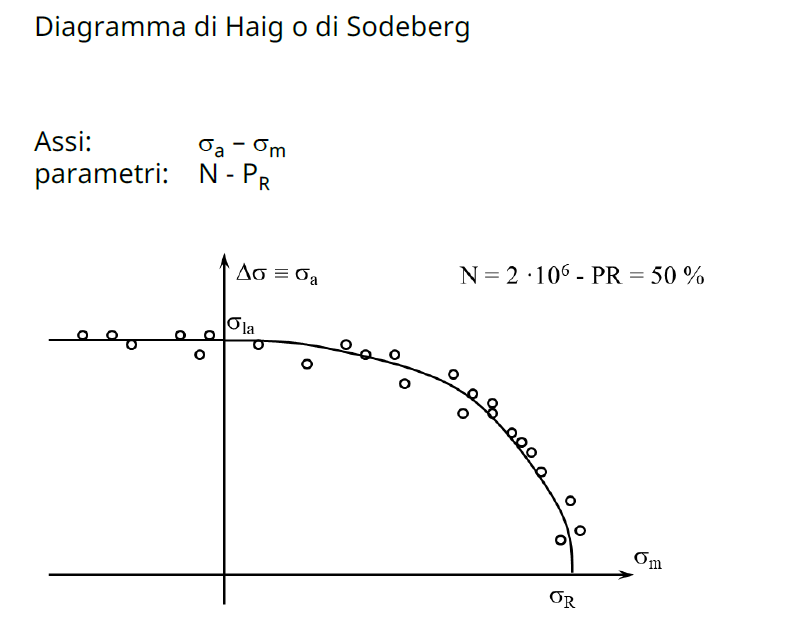
\includegraphics[width=0.5\linewidth]{immagini/screenshot003}
	\label{fig:screenshot003}
\end{figure}		
		
		È più che noto che avendo applicato solo un momento, l'equilibrio a traslazione in direzione $z$ deve risultare nullo:
		\[ N = \int_A\sigma_zdA = k\int_A(d'_nP)dA= kS'_n = 0\]
		Dove con $S'_n$ si è identificato il momento statico espresso in misure oblique. 
		
		Essendo verificato per ipotesi l'equilibrio a traslazione, sarà proprio questo momento statico "obliquo" ad essere nullo, avvalorando così la dimostrazione che $n$ è un asse baricentrico. \newline 
		
		D'altro canto so che il momento intorno ad $s$ anche lui dev'essere nullo perché: (1) ho applicato un momento intorno ad $m$; (2) $s \perp m$ per definizione. 
		
		L'equilibrio a rotazione diviene quindi: 
		\[ M_s = \int_A\sigma_z(d_sP)dA = 0 \]
		
\begin{figure}[H]
	\centering
	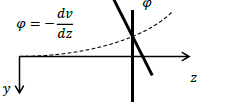
\includegraphics[width=0.5\linewidth]{immagini/screenshot004}
	\label{fig:screenshot004}
\end{figure}

		Scrivendo:
		\[(d_sP) = (d'_sP)\cos\theta\]
		Si giunge a:
		\[ \int_A\sigma_z(d_sP)dA = k\int_A(d'_nP)(d'_sP)\cos\theta dA = k \cdot I'_{ns}\cos\theta\]
		Dove con $I'_{ns}$ si è identificato il momento centrifugo espresso in misure oblique.
		
		Anche qui essendo verificato per ipotesi l'equilibrio a rotazione, sarà proprio questo momento centrifugo "obliquo" ad essere nullo, dimostrando così che gli assi $s$ ed $n$ sono proprio coniugati. \newline 
		
		Applichiamo adesso, infine, l'equilibrio a rotazione intono all'asse $s$, per ipotesi non nullo e uguale al momento deviato imposto: 
		\[M = \int_A\sigma_z(d_mP)dA \]
		
\begin{figure}[H]
	\centering
	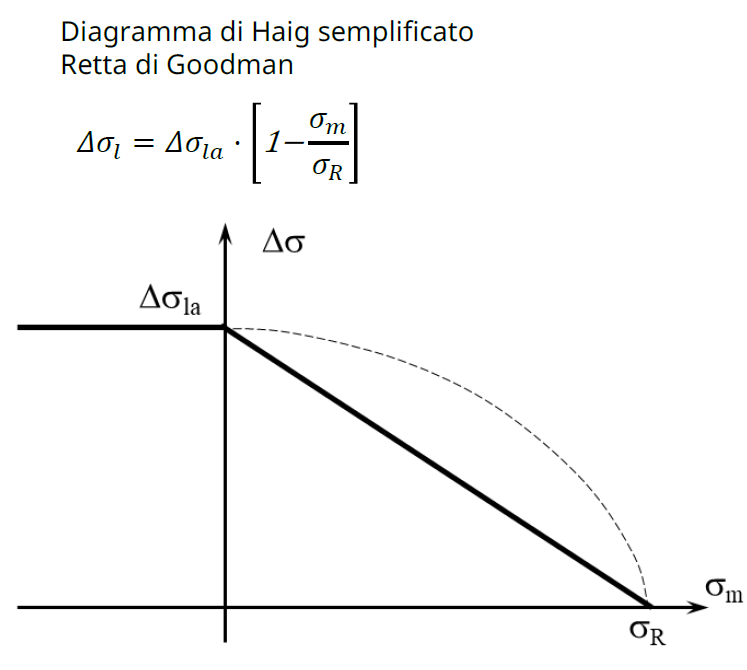
\includegraphics[width=0.4\linewidth]{immagini/screenshot005}
	\label{fig:screenshot005}
\end{figure}

		Scrivendo:
		\[ d_mP = d'_nP + d'_sP\sin\theta\]
		Si giunge a: 
		\[M = \int_Ak(d'_nP)(d'_nP + d'_sP\sin\theta)dA = kI'_n + kI'_{ns}\sin\theta\]
		Poiché poco sopra si è dimostrato che $I'_{ns}=0$:
		\[M=kI'_n \Rightarrow k =\dfrac{M}{I'_n}\]
		
		Si è così infine trovata la funzione che descrive la visualizzazione del momento secondo distanze oblique:
		\[ \sigma_z = \dfrac{M}{I'_n}d'_nP\]
		Tale formula prende il nome di \textbf{Formula Monomia} e può essere manipolata per permettere di tracciare il diagramma delle tensioni su di una fondamentale non più parallela ad $s$ ma ortogonale ad $n$:
		\[ \sigma_z =\dfrac{M}{I'_n}d'_nP \cdot  \dfrac{\cos^2\theta}{\cos^2\theta}= \dfrac{M\cos\theta}{I'_n\cos^2\theta}d'_nP\cos\theta = \dfrac{M_n}{I_n}d_nP\]
		In questo modo non rappresento più il momento in forma obliqua, ma in forma ortogonale rispetto all'asse neutro e la parte di momento di cui terrò conto sarà quella lungo $n$. \newline 
		
		Perché per trovare i valore di momento di flessione non è sufficiente sostituire le coordinate $(x,y$) direttamente in (\ref{eq:1})? La flessione retta era più facilmente visibile e interpretabile, a maggiori $y$ corrispondevano maggiori tensioni; qui no, a meno di sezioni semplici l'andamento del momento non è facilmente leggibile, allora ci si chiede, dov'è la massima tensione? Alla massima distanza dall'asse neutro, scrivendo perciò la relazione monomia si possono trovare i punti più sollecitati e il risultato che ne scaturisce è che questi punti ora li so individuare: una volta trovata l'inclinazione di $n$ traccio due parallele tangenti alla sezione che intersecheranno una fondamentale ortogonale ad $n$. \newline 
		
		Per la linea d'asse le deformazioni risultano essere: 
		\[ \text{Per} ~ M_x \hspace{0.5cm} u = 0 \hspace{0.5cm} v = -\dfrac{1}{2}\dfrac{M_x}{EI_x}z^2 \hspace{0.5cm} w = 0\]
		\[ \text{Per} ~ M_y \hspace{0.5cm} u = \dfrac{1}{2}\dfrac{M_y}{EI_y}z^2 \hspace{0.5cm} v = 0 \hspace{0.5cm} w = 0\]
		\[ \text{Per} ~ M_x +M_y \hspace{0.5cm} u = \dfrac{1}{2}\dfrac{M_y}{EI_y}z^2 \hspace{0.5cm} v = -\dfrac{1}{2}\dfrac{M_x}{EI_x}z^2 \hspace{0.5cm} w = 0\]
		Dove si trova la linea d'asse a seguito di una flessione deviata? Ora l'inflessione è deviata e si trova su di un piano inclinato rispetto ad $x$ ed $y$, in un piano che non è nè $xz$ nè $yz$ ed è individuato dal versore che ha come coseni direttori null'altro che i coefficienti degli spostamenti:
		\[\hat{f} = \left(\dfrac{M_y}{EI_y}; -\dfrac{M_x}{EI_x}\right)\]
		Individua un asse di flessione nel piano di sezione.
		
		Dalla definizione la linea d'asse si inflette secondo un piano ortogonale a quello neutro, che d'altronde ha orientazione data da:
		\[\left( dfrac{M_x}{EI_x};\dfrac{M_y}{EI_y}\right)\]
		E risulta visibilmente ortogonale all'asse di flessione. 
		
		Inoltre si nota che linea d'asse non si allunga e le sezioni rette restano ortogonali all'asse della trave. \newline 
		
		\textbf{{\Large Presso/Tenso - Flessione}} \newline 
		Se si considera l'azione contemporanea di un momento deviato (o di due momenti flettenti retti) e uno sforzo normale, la tensione sarà data dall'equazione:
		\[ \sigma_z = \dfrac{N}{A} + \dfrac{M_x}{I_x}y - \dfrac{M_y}{I_y}x \]
		E l'asse neutro sarà individuato dall'equazione:
		\[ \dfrac{N}{A} + \dfrac{M_x}{I_x}y - \dfrac{M_y}{I_y}x \]
		La sovrapposizione degli effetti può essere sfruttata per definire in questo caso oltre al sistema di forze sopra menzionato, un altro sistema di forze equivalente, un'altra combinazione elastica di momenti e sforzo normale: il caso di un'azione di solo sforzo normale eccentrico applicato in un punto $ C $ detto centro di pressione, diverso dal baricentro, che applica due momenti: 
		\[ M_x = Ne_y \hspace{1cm} M_y = -Ne_x\]
		in questo modo:
		\[ \sigma_z = N\left(\dfrac{1}{A} + \dfrac{e_y}{I_x}y - \dfrac{e_x}{I_y}x\right) \]
\begin{figure}[H]
	\centering
	\label{fig:screenshot006}
	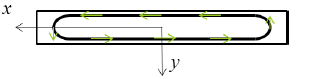
\includegraphics[width=0.2\linewidth]{immagini/screenshot006}
\end{figure}
\newpage		
		\textbf{Ellisse centrale di inerzia} \newline 
		Data una figura $A$ si definisce ellisse centrale di inerzia o ellisse di Culmann del sistema continuo, l'ellisse che ha per centro il baricentro $G$ di $A$ e per semiassi i raggi principali d'inerzia.
		\[ \rho_\xi = \sqrt{\dfrac{I_\xi}{A}} \hspace{1cm} \rho_\eta = \sqrt{\dfrac{I_\eta}{A}} \]
\begin{figure}[H]
	\centering
	\begin{tikzpicture} [>=latex]
	%\draw [thin, help lines] (0,0) grid (5,5);
	\draw (1.5,1) ellipse (2 and 2.5);
	\draw[<->] (1.5,1) -- (3.5,1) node [pos=0.5, below] {$\rho_\xi$};
	\draw[<->] (1.5,1) -- (1.5,3.5) node [pos=0.5, right] {$\rho_\eta$};
\end{tikzpicture}
\end{figure}
	
		Alla massima inerzia corrisponde il semiasse maggiore e viceversa.
		
		L’ellisse
		visualizza sinteticamente le proprietà geometriche della sezione risultando di forma più
		allungata nella direzione di minima inerzia permette di visualizzare dove si sviluppa maggiormente la resistenza inerziale della sezione. \newline 
		
		Un carico applicato equivalente ad una forza applicata in C
		determina delle sollecitazioni che sono date dalla
		sovrapposizione degli effetti:
		\[
		N ~ in ~ C = \begin{cases}
			N \\
			M_x = Ny_C \\
			M_y = -Nx_C
		\end{cases}
		\] 
		E l'asse neutro si può trovare ora in funzione dei raggi d'inerzia: 
		\[ 1+ \dfrac{y_C}{\rho^2_x}y + \dfrac{x_C}{\rho^2_y}x = 0\]
		E diventa una \textit{relazione di coniugio} tra l'asse neutro e quello delle sollecitazioni, tra l'asse neutro e il punto di applicazione $C$ del carico: l'asse neutro si dice retta coniugata rispetto all'ellisse di Culmann del punto $ C $. \newline 
		
		\textit{L'asse neutro è la retta coniugata del punto C nella polarità, avente come conica fondamentale l'ellisse di Culmann della sezione}. \newline 
		
		\textit{Il punto $C$ prende il nome di \textbf{antipolo} e la retta $n$ prende il nome di \textbf{antipolare} del centro $C$ di sollecitazione.} \newline
		
		\textit{Si definisce nocciolo centrale di inerzia (NCI) il luogo degli antipoli delle rette non secanti la sezione
		trasversale della trave.} \newline
		
		\textit{Le rette che rappresentano l'inviluppo convesso della sezione generano la frontiera del nocciolo.}\newline
		
		Allontanandosi dalla retta tangente alla sezione gli antipoli entrano all'interno del NCI. \newline 
		
		Nel caso di sezione rettangolare il NCI corrisponde ad un rombo i cui vertici sono gli antipoli degli assi tangenti i fianchi della sezione, tutti i punti da $A_1$ ad $A_3$ sono gli antipoli delle rette appartenenti al fascio proprio di rette passante per lo spigolo.
		
		Laddove una sezione abbia un fianco rettilineo sarà lì che si avrà un vertice del NCI, laddove ci sarà un vertice della sezione, si avrà invece una linea continua di frontiera del NCI.
		
\begin{figure}[H]
	\centering
	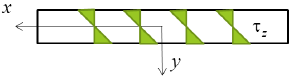
\includegraphics[width=0.7\linewidth]{immagini/screenshot007}
	\label{fig:screenshot007}
\end{figure}

		Si perviene così ad una nuova definizione di frontiera del NCI: 
		
		\hyperref[frontiera]{La frontiera del NCI rappresenta gli antipoli delle rette tangenti.} \newline
		
		È importante il NCI per valutare la pressoflessione. 
		
		La pressofelssione è un elemento cardine nell'ambito civile, è il modo in cui è sollecitata una qualunque colonna (portante): carico verticale + momento o carico verticale eccentrico. 
		
		Ricordi come la flessione deviata generi un asse neutro indipendente dal valore di $M$ ma solo dalla sua inclinazione e dalle caratteristiche della sezione? Ebbene a ciò si aggiunge uno sforzo normale $N/A$, l'asse neutro dipenderà così in questo caso esclusivamente dal punto di applicazione $C$ della forza, perché è antipolare dell'antipolo $C$.
		
		Dato $C$ si può trovare $n$ e viceversa.
		
\begin{figure}[H]
	\centering
	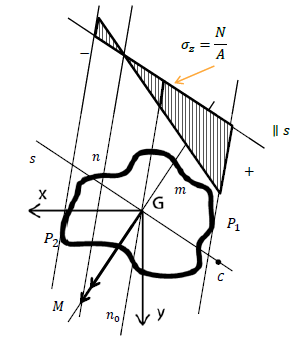
\includegraphics[width=0.5\linewidth]{immagini/screenshot008}
	\label{fig:screenshot008}
\end{figure}

		Si nota infine che il baricentro $G$ si trova sempre in mezzo tra C antipolo ed $n$ antipolare, perché a sua volta l’asse
		neutro si trova sempre, rispetto al baricentro $ G $, dalla parte opposta al centro di
		sollecitazione $ C $; esso si avvicina a $ G $ all’aumentare della distanza di $ C $ da $ G $. \newline 
		
		Se si applica una forza in $A_2$, punto di frontiera del NCI l'asse neutro combacia con $a_2$, un asse neutro tangente implica così l'inesistenza di un andamento a farfalla, la trave in questo modo è sollecitata totalmente a trazione \textbf{O} a compressione, se addirittura si applica una forza all'interno del NCI, l'asse neutro si sposta all'esterno della sezione! Se poi
		il punto di applicazione $ C $ coincide con il baricentro, l’asse neutro esplode all’infinito e ci si riconduce al solo sforzo
		normale. \newline
		
%IMAG nocciolo modificata con diagramma modificato
	
		Tutta la struttura è così caricata da tensioni di un solo segno, che è meglio di un andamento a farfalla soprattutto per materiali non isotropi, che non hanno lo stesso comportamento a trazione o compressione. 
		
		Infatti per una colonna, quello che si fa per far cadere il carico nel all'interno del NCI, è piazzare due architravi equamente caricati così da bilanciare il contributo del carico sovrastante. \newline 
		
		Infine, la linea d'asse della pressoflessione si inflette secondo un piano di sezione che segue le regole della flessione deviata, quindi ortogonalmente al piano neutro, ed in più subisce un allungamento o compressione dovuto allo sforzo normale aggiunto. 
		
		
		
		
	
		
		
		
		
		
		
		
		
		 
		
		
		
	\newpage
	{\Large \textbf{NOTE}}
%	\vfill
%\begin{tcolorbox}[height=4.5cm]
%	This box has a height of 4.5cm.
%\end{tcolorbox}

%DA DECOMMENTARE PER AVERE LA VERSIONE STAMPABILE A DUE PAGINE 	
%	\newpage
%		\null
%		\vfill
%\begin{tcolorbox}[height=4.5cm]
%	This box has a height of 4.5cm.
%\end{tcolorbox}
%		
\end{adjustwidth}
\end{document}
\documentclass{article}
\usepackage[left=0.85in, right=0.85in, top=0.5in, bottom=0.95in]{geometry}
\usepackage[T1]{fontenc}
\usepackage[utf8]{inputenc}
\usepackage[italian]{babel}
\usepackage{graphicx}
\usepackage{wrapfig2}
\usepackage{amsmath}
\usepackage{amssymb}
\usepackage{cases}
\usepackage{gensymb} %simboli come ° = \degree  etc etc
\usepackage{subcaption}
\usepackage{hyperref}
\hypersetup{
	colorlinks=true,
	linkcolor=blue,    
	urlcolor=blue,
	%pdfpagemode=FullScreen,
}
\urlstyle{same}
\usepackage{changepage}
\usepackage{lastpage, epstopdf}
\usepackage{fancyhdr}
\usepackage{tcolorbox}
\usepackage{background}
\usepackage{tikz}
\usetikzlibrary{patterns}


%=======HEADER & FOOTER=======%
\def\lesson{Lezione N. 5}
\def\outcome{\textbf{Learning Outcomes:} Outcomes go here. }

\pagestyle{fancy}
\fancyhf{}
\renewcommand{\headrulewidth}{0pt}
\renewcommand{\footrulewidth}{1.4pt}
\lfoot{A.M. $\diamond$ \the\year}
\cfoot{Page \thepage}
\rfoot{\lesson}

%=======CORNELL STYLE FORMAT=======%
\SetBgScale{1}
\SetBgAngle{0}
\SetBgColor{black}
\SetBgContents{\rule{1pt}{0.85\paperheight}}
\SetBgHshift{-1.6in}
\SetBgVshift{-0.1in}

%=======CUSTOM BOXES=======%

\parindent 0ex

%=======BODY=======%
\begin{document}
	\setcounterpageref{secnumdepth}{0}
	\section*{Parte 5} %Date: \hrulefill}
%	\begin{tcolorbox}{\outcome}\end{tcolorbox}

\begin{adjustwidth}{2in}{} 
	
\textbf{{\Large De Saint Venant: Torsione}} \mbox{} \newline
		Ci si ponga nel caso in cui sulla faccia terminale della trave venga posto un momento torcente, questo genererà uno spostamento che non interesserà la linea d'asse, e quindi uno spostamento nullo dell'asse baricentrico: la sezione esce dal piano $xz$, il problema non è più piano. \newline 
		
		Le soluzioni esatte in forma chiusa per questo tipo di problema esistono solo per sezioni polari o per sezioni ellittiche o poligonali regolari, per altre sezioni ci si accontenta di una soluzione approssimata ma sicura. \newline 
		
		\item[$\rightarrow$] Per sezioni compatte la distribuzione di massa è intorno al baricentro, ed esistono alcune soluzioni esatte;
		\item[$\rightarrow$] Per sezioni in parete sottile che siano aperte o chiuse la soluzione è approssimata. 
		
		Si ipotizzi perciò di avere una trave a sezione circolare, a simmetria polare, secondo le ipotesi che le sezioni rette ortogonali all'asse medio rimangano rette ortogonali all'asse medio, a seguito di un momento torcente ottengo una rotazione della trave, e a seguito di una rotazione è ben noto che un punto sulla sezione si muove su $x$ ed $y$.
		
\begin{figure}[H]
	\centering
	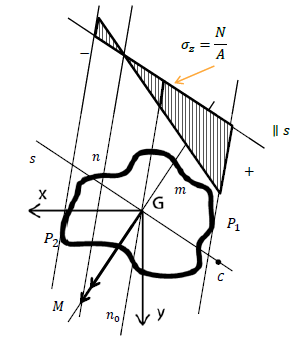
\includegraphics[width=0.5\linewidth]{immagini/screenshot008}
	\label{fig:screenshot008}
\end{figure}

		La rotazione della sezione intorno a $z$ sarà null'altro che proporzionale a $z$ per cui a $z=0$ la rotazione è nulla mentre a $z=l$ la rotazione è massima, l'aliquota di rotazione sarà perciò data da: 
		\[ \theta = \theta(z)= \Theta z\]
		Dove $\Theta$ è l'angolo unitario di torsione (AUT) e tiene conto della rotazione tra due facce contigue poste a distanza infinitesima.
		\[\Theta - \dfrac{\partial \theta}{\partial z}\]
		
		Per lo studio di questo problema si applica il metodo semi-inverso agli spostamenti, per cui per piccoli spostamenti, $u, v, w$ devono combaciare con la rotazione piana:

\begin{figure}[H]
	\centering
	\begin{tikzpicture} [>=latex]
		%\draw [thin, help lines] (0,0) grid (5,5);
		\draw [thick, ->] (0,0) -- (4,0) node [pos = 1, right] {$x$};
		\draw [thick, ->] (0,0) -- (0,4) node [pos = 1, above] {$y$};
		\draw[->] (0.5,0.5) arc (0:25:3) node [pos = 0.5, right] {$\theta$}; 
		\draw [thick,] (0,0) -- (3,2); 
		\draw [thin, <->] (3,0) -- (3,2)  node [pos = 0.5, right] {$v = \theta x$};
		\draw [thick,] (0,0) -- (-2,2); 
		\draw [thin, <->] (0,2) -- (-2,2)  node [pos = 0.5, above] {$u = -\theta y$};
	\end{tikzpicture}
\end{figure}

		\[ \begin{cases}
			u = -\theta y = -\Theta yz \\
			v = \theta x = \Theta xz \\
			w = 0
		\end{cases}\]
		Da questi spostamenti è possibile ricavare un campo di tensioni che soddisfi l'equilibrio?
		\[ 
	\begin{cases}
		\begin{aligned}
			\varepsilon_{xx} =   \frac{\partial u_x}{\partial x} = \dfrac{1}{E}[\sigma_x - \nu(\sigma_y + \sigma_z)] = 0 \\
			\varepsilon_{yy} =   \frac{\partial u_y}{\partial y} = \dfrac{1}{E}[\sigma_y - \nu(\sigma_x + \sigma_z)] = 0 \\
			\varepsilon_{zz} =   \frac{\partial u_z}{\partial z} = \dfrac{1}{E}[\sigma_z - \nu(\sigma_x + \sigma_y)] = 0 \\
		\end{aligned}
	\end{cases} \hspace{0.2cm} \begin{cases}
		\begin{aligned}
			\gamma_{xy} =   \frac{\partial u_y}{\partial x} + \frac{\partial u_x}{\partial y} = \dfrac{1}{G} \tau_{xy} = -\Theta z + \Theta z = 0\\
			\gamma_{yz} =   \frac{\partial u_y}{\partial z} + \frac{\partial u_z}{\partial y} = \dfrac{1}{G} \tau_{xz} = -\Theta y \\
			\gamma_{zx} =   \frac{\partial u_z}{\partial x} + \frac{\partial u_x}{\partial z} = \dfrac{1}{G} \tau_{yz} = \Theta x \\
		\end{aligned}
	\end{cases}
		\]
		Le dilatazione sono nulle, così come le distorsioni $\gamma_{xy}$, ma lo stesso non si può dire per le distorsioni $\gamma_{zx}$ e $\gamma_{yz}$, entrambe non nulle. \newline 
	
		Il che si traduce nell'avere la completa assenza di azioni normali, queste soppiantate dalle sole azioni tangenziali, la torsione genera soltanto tensioni di tipo tangenziale: 
		\[ \tau_{xz} = -G\Theta y \hspace{1cm} \tau_{yz} = G\Theta x\]
		Il tensore delle tensioni diviene così: 
	 	\[ \left[ \begin{array}{ccc}
		0 & 0 & -G\Theta y \\
		0 & 0 & G\Theta x \\
		-G\Theta y & G\Theta x & 0
		\end{array}\right] \]
		Si verifichi adesso il problema di De Saint Venant attraverso gli equilibri. 
		
		Per gli equilibri interni le condizioni indefinite di equilibrio risultano immediatamente soddisfatte, col risultato che il campo di tensioni risulta piano (sempre per quel discorso che $\det[\sigma]\equiv\Rightarrow\exists$ almeno due soluzioni) 
		\[
		\begin{cases}
			\begin{aligned}
				\frac{\partial \tau_{zx}}{\partial z} & =0 \\
				
				\frac{\partial \tau_{zy}}{\partial z} & =0 \\
				
				\frac{\partial \tau_{xz}}{\partial x} + \frac{\partial \tau_{yz}}{\partial y} + \frac{\partial\sigma_z}{\partial z} & =0 \\
			\end{aligned}
		\end{cases}
		\]
		Le condizioni al contorno si trasformano in:
		\[ \tau_{xz}n_x + \tau_{yz}n_y = 0\]
		Si è dimostrato in questo modo come il vettore tensione sia ortogonale alla normale
		della giacitura coincidente la superficie tangente al
		bordo della sezione nel punto in esame, perché banalmente, se $n_x, n_y$ sono co coseni direttori della normale e il vettore tensione si può scrivere secondo le sue componenti $\vec{\tau}_z = (\tau_{xz}\hat{i} +  \tau_{yz}\hat{j})$, allora:
		\[\vec{\tau}_z \cdot \hat{n} = 0\]
		Nel caso specifico di sezione circolare, si può scrivere questa relazioni in termini di raggio, d'altronde è ben noto che in una sezione siffatta la normale è radiale, per cui: 
		\[\hat{n} = \vec{R} = x\hat{i} + y\hat{j}\]
		A allora varrà ugualmente che la direzione del vettore tensione sarà sempre ortogonale al vettore posizione, che in una sezione circolare corrisponde ad una variabile radiale:
		\[\vec{\tau}_z \cdot \vec{R} = 0 \Rightarrow \tau_{xz}x +  \tau_{yz}y = 0 \Rightarrow -G\Theta yx + G\Theta xy =0 \]
		\[ G\Theta yx = G\Theta xy \]
		Si è così al cospetto della soluzione esatta. 
		
		Tutti
		punti sullo stesso diametro hanno un vettore tensione con direzione costante e modulo
		proporzionale alla distanza dall’asse di rotazione.\newline 
		
		\item\textbf{Osservazione}\newline 		
			$\vec{\tau}_z$ è tangente al bordo, ma in una sezione circolare questo significa che è sempre ortogonale al raggio: avrà sempre direzione circonferenziale rispetto al sistema di riferimento, ovvero esiste una linea di flusso di $\tau$ che si chiude lungo tutto il bordo, è una circonferenza, un luogo di punti caratterizzato dalla stessa tensione, dalla stessa intensità del vettore tensione, in cui è sempre uniforme in modulo ma non in direzione e verso, queste dettate dalla tangenza della linea di flusso stessa.
			
\begin{figure}[H]
	\centering
	\begin{tikzpicture} [>=latex]
		%\draw [thin, help lines] (0,0) grid (5,5);
		\draw (2.5,2.5) circle (2.5 and 2.5);
		\draw[->] (2.5,2.5) -- (3.5,2.5) node [pos=1, right] {$x$};
		\draw[->] (2.5,2.5) -- (2.5,3.5) node [pos=1, above] {$y$};
		%\draw (0.75,0.75) -- (4.25,4.25);
		%\draw [rotate around={30:(2.5,2.5)}] (0.75,0.75) -- (4.25,4.25);
		\draw[pattern=vertical lines] (4.25,4.25) -- (3.14, 4.91) -- (2.5,2.5) -- (4.25,4.25);
		\draw[pattern=vertical lines] (0.75,0.75) -- (1.89, 0.09) -- (2.5,2.5) -- (0.75,0.75);
		
		\foreach \angle in {0, 30, 60, 90, 120, 150, 180, 210, 240, 270, 300, 330}
		{
			\pgfmathsetmacro{\x}{2.5 + 2.5 * cos(\angle)}
			\pgfmathsetmacro{\y}{2.5 + 2.5 * sin(\angle)}
			\draw[->] (\x, \y) -- ++({-sin(\angle)}, {cos(\angle)});
		}
	\end{tikzpicture}
\end{figure}

			Le linee di flusso del vettore tensione sono circonferenze
			concentriche con la circonferenza che individua il bordo
			della sezione retta.
			
			Il diagramma in esame inoltre fornisce la vera rappresentazione del vettore tensione! Col momento torcente, a differenza del momento flettente, so rappresentando direzione, verso, e intensità sullo stesso diagramma.
			\[ |\vec{\tau}_z| = \sqrt{\tau^2_{xz} + \tau^2_{yz}} = G\Theta\sqrt{x^2 + y^2} = G\Theta r\]
			$\vec{\tau}_z$ è in questo modo linearmente dipendente dalla quota radiale, oltre che essere ortogonale a $\vec{R}$. \newline 
			
			Il problema però è che ancora non so determinare l'angolo unitario di torsione $\Theta$. 
			
			Mi corrono in soccorso le caratteristiche della sollecitazione, di cui però si è già ricavato le tensioni, si vede subito che le uniche caratteristiche che interessano la trattazione sono: 
			caratteristiche della sollecitazione sulla $S_l$ perciò saranno:
			\[\begin{matrix}
				\begin{aligned}
					T_x = \int_A \tau_{zx}dA = -G\Theta\int_AydA = -G\Theta S_x = 0 &  \\
					T_y = \int_A \tau_{zy}dA = G\Theta\int_AxdA = G\Theta S_y =0 \hspace{1cm} &  M_z = \int_A (\tau_{zy}x -\tau_{zx}y)dA
				\end{aligned}	
			\end{matrix}\]
			Dove gli $S_i$ sono nulli per la classica ipotesi di sistema riferimento baricentrale, il momento $M_z$ per rispettare l'equilibrio, dovrà proprio essere uguale al momento torcente:
			\[ M_z = M_t = \int_A (\tau_{zy}x -\tau_{zx}y)dA = G\Theta\int_Ax^2dA + G\Theta\int_Ay^2dA = G\Theta\int_A(x^2 + y^2)dA = G\Theta I_z \]
			Dove si è identificato con $I_z$ il momento d'inerzia polare, rispetto all'asse ortogonale alla sezione stessa, somma dei contributi di momento d'inerzia su $x$ ed $y$. \newline
			
			Da quest'ultima relazione so così finalmente trovarmi l'angolo $\Theta$: 
			\[ \Theta = \dfrac{M_t}{GI_z}\]
			in cui $GI_z$ è il modulo di rigidezza torsionale. \newline 
			
			Quest'angolo si può immediatamente sostituire negli spostamenti e nelle tensioni ottenendo: 
			\[ \begin{cases}
				u = -\Theta yz = -\dfrac{M_t}{GI_z}yz \\
				v =  \Theta xz = \dfrac{M_t}{GI_z} xz\\
				w = 0
			\end{cases} \hspace{0.3cm} \tau_{xz} = -G\Theta y = -\dfrac{M_t}{I_z}y  \hspace{0.3cm} \tau_{yz} = G\Theta x = \dfrac{M_t}{I_z}x\]
			La rotazione infine sarà data da quella della faccia finale meno quella della faccia iniziale, se la rotazione era definita come $\theta = \Theta z$ e se per ipotesi la rotazione sulla faccia iniziale era data nulla, si ha: 
			\[\Delta\theta = \theta(L) - \theta(0) = \theta(L) = \dfrac{M_t}{GI_z}L\]
			Infine, matematicamente l'inerzia polare per una sezione circolare può essere scritta come: 
			\[ I_z = \int_A r^2dA = \dfrac{\pi R^4}{2}\]
			Così, se nella sua forma finale $|\vec{\tau}_z| = G\Theta r$, si potrà scrivere:
			\[ \boxed{\tau_z = \dfrac{M_t}{GI_z}r = \dfrac{2M_t}{\pi R^4}r} \]
			\begin{figure}[H]
				\centering
				\includegraphics[width=0.2\linewidth]{immagini/screenshot002}
				\label{fig:screenshot002}
			\end{figure}
			
			Si vede immediatamente che le tensioni massime si genereranno al bordo esterno della sezione retta.\newline 
			
			Tale modello sarà perfettamente riproducibile (a meno di sezione assialsimmetrica) anche al caso di sezioni circolari cave, in cui l’unico aspetto
			modificato risulta il valore del momento di inerzia polare, ma valendo i principi booleani di somma e sottrazione delle aree si possono senza problemi combinare le rispettive inerzie delle sezioni: 
			\[ \boxed{\tau_z = \dfrac{2M_t}{\pi (R_{ext}^4-R_{int}^4)}r} \]
			
\begin{figure}[H]
	\centering
	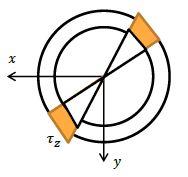
\includegraphics[width=0.2\linewidth]{immagini/screenshot001}
	\label{fig:screenshot001}
\end{figure}


			Quando lo spessore della parete diminuisce, la differenza tra il vettore tensione al raggio esterno e quello al raggio interno diviene decisamente trascurabile, si perviene in questo modo a soluzioni ancor più semplificate che prevederanno una costanza di $\tau$ lungo tutto lo spessore. \newline

		\textbf{{\Large Sezione generica}} \newline 
		La soluzione precedente non è però applicabile ad una sezione generica. 
\begin{figure}[H]
	\centering
	\label{fig:screenshot003}
	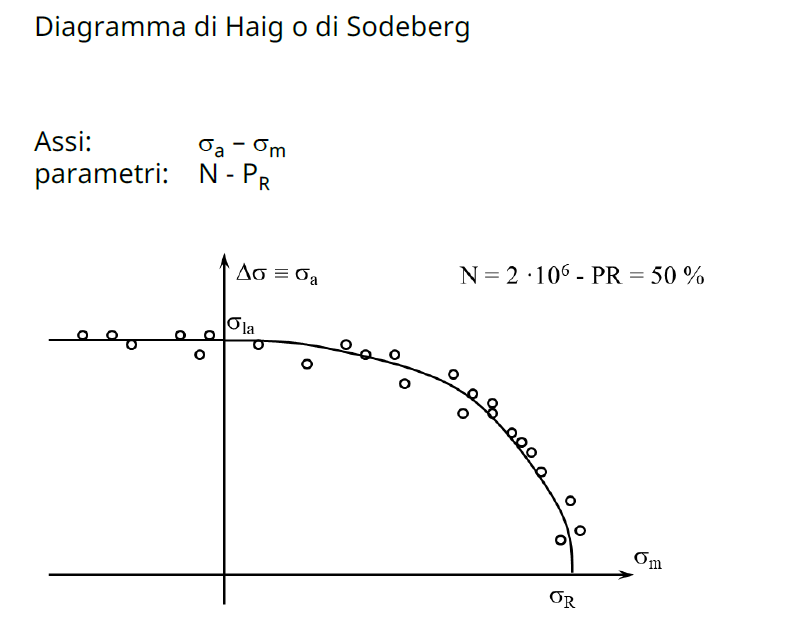
\includegraphics[width=0.5\linewidth]{immagini/screenshot003}
\end{figure}
		Ad esempio, una $\tau$ circonferenziale non soddisfa più le condizioni al contorno di ortogonalità in tutti i punti del bordo, è dunque necessario cercare una nuova soluzione o modificare quella precedente.
		
		Si mettono dei paletti ad $u$ e $v$, questi sono intoccabili e garantiscono che la sezione ruoti in modo uniforme senza separazione di materiale, rimuovo allora l'ipotesi che le sezioni piane rimangano piane. 
		
		Attribuisco così a $w$ una funzione $\omega(x,y)$, dipendente dalla specifica forma della sezione, che mi dirà lo spostamento in $z$ essere concesso. 
		
		Tale spostamento lo si proporzionerà all'angolo unitario di torsione e lo si definisce per ipotesi costante in $z$: tutte le sezioni si sposteranno della stessa quantità, a seguito della torsione le fibre si muoveranno in direzione $z$ ognuna in modo differenziato.
		
		\textbf{NB:} Le fibre si spostano soltanto in direzione $z$, non si dilatano, la forma della sezione rimarrà la stessa, è come si si lasciasse un'impronta su di una faccia estremale di cui si troverà il negativo sulla faccia estremale opposta, l'impronta è proprio la funzione ingobbamento, che si ritroverà esattamente identica in tutte le sezioni della trave, fino alla faccia frontale.  		
		\[ \varepsilon_{zz} = \dfrac{\partial w}{\partial z} = 0 \Rightarrow \begin{cases}
			u = -\Theta yz  \\
			v =  \Theta xz  \\
			w = \Theta \omega(x,y)
		\end{cases} \]
		Avendo rimosso così la simmetria polare, ci si aspetta
		che la sezione trasversale presenti un \textbf{ingobbamento $\omega(x,y)$},
		costante per tutte le sezioni.\newline 
		
		Come definisco le tensioni? 
		\[ 
		\begin{cases}
			\begin{aligned}
				\varepsilon_{xx} =   \frac{\partial u_x}{\partial x} = 0 \\
				\varepsilon_{yy} =   \frac{\partial u_y}{\partial y} = 0 \\
				\varepsilon_{zz} =   \frac{\partial u_z}{\partial z} = 0 \\
			\end{aligned}
		\end{cases} \hspace{0.2cm} \begin{cases}
			\begin{aligned}
				\gamma_{xy} =   \frac{\partial u_y}{\partial x} + \frac{\partial u_x}{\partial y} = -\Theta z + \Theta z = 0\\
				\gamma_{yz} =   \frac{\partial u_y}{\partial z} + \frac{\partial u_z}{\partial y} = \dfrac{1}{G} \tau_{xz} = \Theta \left(\dfrac{\partial \omega}{\partial x}-y\right) \\
				\gamma_{zx} =   \frac{\partial u_z}{\partial x} + \frac{\partial u_x}{\partial z} = \dfrac{1}{G} \tau_{yz} = \Theta \left(\dfrac{\partial \omega}{\partial y} + x\right)\\
			\end{aligned}
		\end{cases}
		\]
		Lo stato tensionale deve rispettare l’equilibrio interno al volume:
		\[
		\begin{cases}
			\begin{aligned}
				\frac{\partial \tau_{zx}}{\partial z} & =0 \\
				
				\frac{\partial \tau_{zy}}{\partial z} & =0 \\
				
				\frac{\partial \tau_{xz}}{\partial x} + \frac{\partial \tau_{yz}}{\partial y} + \frac{\partial\sigma_z}{\partial z} & = \frac{\partial \tau_{xz}}{\partial x} + \frac{\partial \tau_{yz}}{\partial y} = \vec{\nabla}\cdot\vec{\tau}_z = 0 \\
			\end{aligned}
		\end{cases}
		\]
		Quello che si ottiene e che, affinché venga verificata l'ultima equazione, deve valere:
		\[ \vec{\nabla}\cdot\vec{\tau}_z = 0 \]
		\[G\Theta\left(\dfrac{\partial^2 \omega}{\partial y^2} + \dfrac{\partial^2 \omega}{\partial x^2} \right)= 0\]
		Vera se e solo se:
		\[ \boxed{\dfrac{\partial^2 \omega}{\partial y^2} + \dfrac{\partial^2 \omega}{\partial x^2} = 0} \]
		Ovvero se la funzione ingobbamento è una funzione armonica. \newline 
		
		Quello che cambia ora è che l'equilibrio non è più identicamente dimostrato dalla semplice sostituzione delle $\tau$, anzi, è funzione dell'ingobbamento stesso! \newline 
		
		Si verifichino ora le condizioni al contorno che per la torsione abbiamo imparato a sintetizzare come: 
		\[\vec{\tau}_z \cdot \hat{n} = 0\]
		Questa vera se e solo se: 
		\[ G\Theta \left[\left(\dfrac{\partial \omega}{\partial x} - y\right)n_x + \left(\dfrac{\partial \omega}{\partial y} +x\right)n_y\right] = 0\]
		\[ \dfrac{\partial \omega}{\partial x}n_x + \dfrac{\partial \omega}{\partial y}n_y - yn_x  + xn_y = 0\]
		In forma vettoriale $n_x, n_y$ identificano i coseni direttori della normale alla superficie, $,x,y$ identificano il vettore radiale, mentre $ -n_y, n_x$ identificano il vettore tangenziale.
		
\begin{figure}[H]
	\centering
	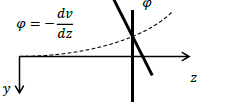
\includegraphics[width=0.5\linewidth]{immagini/screenshot004}
	\label{fig:screenshot004}
\end{figure}
		
		\[ \vec{\nabla}\omega \cdot \hat{n} - \hat{r} \cdot \hat{t} = 0\]
		Si sfritti ora la proprietà del gradiente per il quale se si cambiano le coppie di assi rispetto alle quali si effettuano le derivate parziali, il valore del gradiente non cambia, per cui:
		\[ \left(\dfrac{\partial \omega}{\partial t}, \dfrac{\partial \omega}{\partial n} \right)\cdot \hat{n} - \hat{r} \cdot \hat{t} = 0\]
		Vera se e solo se: 
		\[ \boxed{\dfrac{\partial \omega}{\partial n} = \hat{r} \cdot \hat{t}}\]
		La determinazione della funzione di
		ingobbamento prende il nome di problema di Neumann, che si risolve in forma chiusa per poche sezioni. \newline 
		
		Si dimostri adesso, tramite le caratteristiche della sollecitazione, che tale condizione al contorno appena trovata sia verificata. 
		\[ \begin{split} T_x & = \int_A \tau_{zx}dA =  \int_A\underbrace{\left(\dfrac{\partial}{\partial x}(x\tau_{zx}) -x\dfrac{\partial\tau_{zx}}{\partial x}\right)}_\text{$\dfrac{\partial}{\partial x}(x\tau_{zx}) = 1\tau_{zx} +x\dfrac{\partial\tau_{zx}}{\partial x}$}dA = \\
		& = \int_A \left(\dfrac{\partial}{\partial x}(x\tau_{zx}) -x\left(\dfrac{\partial\tau_{zx}}{\partial x} \underbrace{+ \dfrac{\partial\tau_{zy}}{\partial y} - \dfrac{\partial\tau_{zy}}{\partial y}}_\text{Sommo e Sottraggo}\right)\right) = \\
		& = \int_A\left(\dfrac{\partial}{\partial x }(x\tau_{zx}) + \dfrac{\partial}{\partial y}(x\tau_{zy})\right) = \\ 
		& = \int_{\partial A} x(\tau_{zx}n_x + \tau_{zy}n_y)ds = \int_{\partial A} x(\vec{\tau}\cdot \hat{n})ds = 0	\end{split}\]
		Dove ci si è ricordati che $\dfrac{\partial\tau_{zx}}{\partial x} + \dfrac{\partial\tau_{zy}}{\partial y} =0$. \newline 
		
		Similmente varrà: 
		\[ T_x = \int_A \tau_{zy}dA = 0 \]	
		
		Per il momento invece, so che è pari al momento torcente imposto: 
		\[ \begin{split}
			M_z & = M_t = \int_A (\tau_{zy}x -\tau_{zx}y)dA = G\Theta\int_A \left(x^2 + y^2 + x\dfrac{\partial\omega}{\partial y} - y\dfrac{\partial\omega}{\partial x}\right)dA = \\
			& = G\Theta \left[ I_z + \int_A \left(x\dfrac{\partial\omega}{\partial y} - y\dfrac{\partial\omega}{\partial x}\right)dA \right]
		\end{split} = G\Theta J_t\]
		Con $J_t$ inerzia torsionale.
		
		L'angolo incognito diviene così funzione dell'inerzia torsionale, funzione essa di un integrale geometrico dell'ingobbamento: 
		\[ \Theta = \dfrac{M_t}{GJ_t}\]
		Ci si riconduce così ai casi in cui $\omega = 0$ e l'inerzia torsionale coincide con l'inerzia polare e la sezione e circolare e nel caso generico dove $\omega\neq 0$ ed è necessario calcolare la funzione ingobbamento attraverso il problema di Neumann. \newline 
		
		Si ottiene così, per spostamenti e tensioni: 
			\[ \begin{cases}
			u = -\Theta yz = -\dfrac{M_t}{GJ_t}yz \\
			v =  \Theta xz = \dfrac{M_t}{GJ_t}xz\\
			w = \dfrac{M_t}{GJ_t}\omega(x,y)
		\end{cases} \hspace{1cm} \begin{aligned}
		\tau_{xz} &= G\Theta \left(\dfrac{\partial \omega}{\partial x}-y\right) =\dfrac{M_t}{J_t}  \left(\dfrac{\partial \omega}{\partial x}-y\right) \\
		\tau_{yz} &= G \Theta \left(\dfrac{\partial \omega}{\partial y} + x\right) = \dfrac{M_t}{J_t} \left(\dfrac{\partial \omega}{\partial y} + x\right)
	\end{aligned}\]
	Non importa più per quale asse o punto applico il momento di torsione ora, può essere anche non baricentrico, lo stato tensionale sarà del tutto identico a quello ricavato secondo l'asse baricentrico. 
	
	Applicando il momento torcente per un asse parallelo a $z$ e non baricentrico, le tensioni che si ricavano sono esattamente identiche a quelle ricavate applicando lo stesso momento intorno all'asse $z$ baricentrico. \newline 
	
	La funzione ingobbamento si trova solo per determinate sezioni, le cui tensioni sono rispettivamente: 
	\[\begin{array}{cc}
		\text{Sezione ellittica} & \text{Sezione triangolare} \\ 
		\tau_{xz} = -\dfrac{2M_t}{\pi pq^3}y; \tau_{yz} = \dfrac{2M_t}{\pi pq^3}x  & \tau_{z, max} = \dfrac{M_t}{0.2Ad}  
	\end{array}\]
   \[\begin{array}{ccc}
   	\text{Sezione quadrata} & \text{Sezione esagonale} & \text{Sezione ottagonale} \\
   	\tau_{z, max} = \dfrac{M_t}{0.208Ad} & \tau_{z, max} = \dfrac{M_t}{0.217Ad} & \tau_{z, max} = \dfrac{M_t}{0.223Ad}
   \end{array}\]
			Con $p,q$ semiassi dell'ellisse e $d$ diametro del cerchio iscritto. \newline 
			
			\textbf{Considerazioni}\newline 
			Se è vero che non si può trovare la soluzione in forma chiusa, è anche vero che in qualche modo le tensioni e le sollecitazioni andranno ricavate. 
			
			L'ingobbamento porta con se due fatti notevoli, il primo deriva dall'equazione dell'equilibrio interno $\vec{\nabla} \cdot \vec{\tau} = 0$ mentre il secondo dall'equilibrio al contorno $\vec{\tau} \cdot \hat{n}=0$, tutto ciò si può riassumere dicendo che le linee di flusso appartenenti ad una sezione qualunque sono chiuse, con il notevole risultato di avere un campo di tensione solenoidale: esisterà un luogo dei punti descritto da una curva chiusa caratterizzata da tensioni in modulo identico e direzione tangenziale rispetto a tale curva, con verso imposto dal momento torcente.\newline

			 Inoltre, girando, il campo mi assicura un rotore diverso da zero, costante sul volume e costante rispetto a $z$:
			 \[\vec{\nabla} \times \vec{\tau} = G\Theta \left[\left(\dfrac{\partial^2\omega}{\partial y \partial x} + 1\right) - \left(\dfrac{\partial^2\omega}{\partial x \partial y} - 1\right)\right]\hat{k} = 2G\Theta\hat{k}\]
			 Dove è proprio Schwarz ad assicurarmi che le derivate incrociate sono uguali perché cambiando ordine di derivazione il risultato non cambia. \newline 
			 
			 I vettori di flusso si comportano come i vettori di velocità in un fluido in rotazione, dove c'è restrizione le linee di flusso si avvicinano provocando una tensione tangenziale maggiore, e viceversa, dove c'è allargamento le linee di flusso si diradano e la tensione diminuisce. \newline 
			 
			 Inoltre nelle sezioni
			 sottili chiuse le tensioni tangenziali sono parallele alla linea media e distribuite
			 uniformemente lungo lo spessore mentre nelle sezioni sottili aperte sono parallele alla linea media e variano
			 linearmente lungo lo spessore (valori massimi ai bordi e nulli sulla linea media). \newline
			 
			 \textbf{{\Large Sezione rettangolare sottile aperta}}\newline
			 \textit{Una sezione è aperta se la sua linea media non si chiude. }\newline
			 
			 La sezione rettangolare sottile è un primo esempio di forte approssimazione data da un forte errore di equilibrio, che però non è tuttavia così importante ai fini delle sollecitazione massime.  
			 
\begin{figure}[H]
	\centering
	\label{fig:screenshot005}
	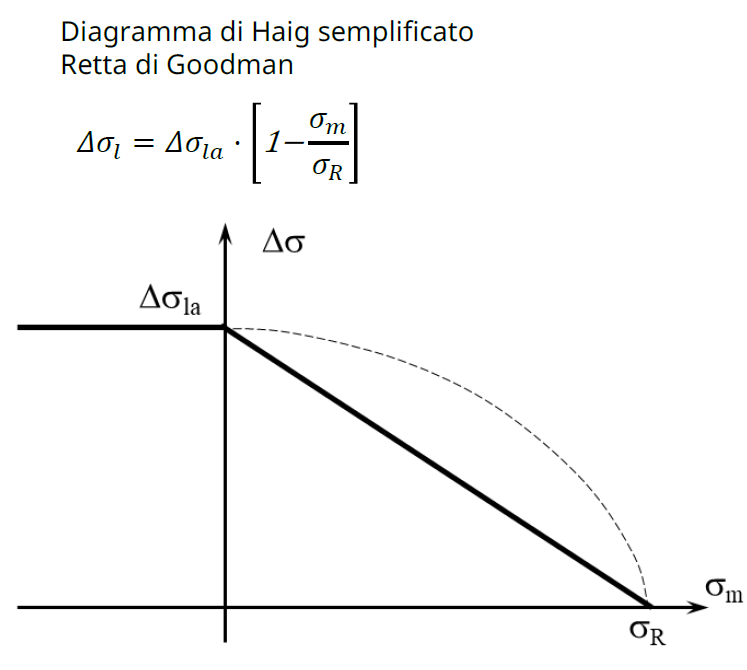
\includegraphics[width=0.5\linewidth]{immagini/screenshot005}
\end{figure}

		
			 Nella sezione circolare il vettore $\tau$ era sempre parallelo alla parete. Se lo spessore lo permetteva, un'altra linea di flusso più interna prevedeva anch'essa vettori paralleli a quella esterna di modulo identico, il che stava a significare un vettore $\tau$ costate lungo tutto lo spessore.  
			 
			 \begin{figure}[H]
			 	\centering
			 	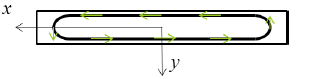
\includegraphics[width=0.5\linewidth]{immagini/screenshot006}
			 	\label{fig:screenshot006}
			 \end{figure}
			 
			 Nel caso di sezioni sottili aperte invece, al $\tau$ sono associate alla stessa quota, sì gli stessi valori, ma opposti, col risultato di un andamento dipendente dallo spessore. Inoltre, come si vede, a parte nelle sezioni estremali, le tensioni sono sempre parallele ai lati lunghi della sezione, per cui a meno di quelle singolarità posso considerare senza - forse - commettere troppi errori:
			 \[ \tau_{zx} = \tau_z\]
			 Con un andamento che dipende da $y$, come detto. 
			 
\begin{figure}[H]
	\centering
	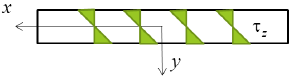
\includegraphics[width=0.5\linewidth]{immagini/screenshot007}
	\label{fig:screenshot007}
\end{figure}

			Se esistono soluzioni di Neumann per una trave quadrata allora esisteranno anche per travi rettangolari, queste sono date da:
			\begin{equation} 
				\label{taumax}
				\tau_{z, max} = \dfrac{M_t}{\dfrac{1}{3}l\delta^2} 
			\end{equation}
			\[ \tau_{xz} = -2\dfrac{M_t}{J_t}y \hspace{0.5cm} J_t = \dfrac{1}{3}l\delta^2 \hspace{1cm} \tau_{zx, max} = \dfrac{M_t}{J_t}\delta \hspace{1cm} \Theta = \dfrac{M_t}{GJ_t} \]
			È questa una soluzione che soddisfa tutte le condizioni? No, è approssimata, tale approssimazione si nota dall'equilibrio delle sollecitazioni, integro il contributo della tensione dovuto alla distribuzione:
			\[ M_z = \int_A(-\tau_{zx}y)dA = \int_A2\dfrac{M_t}{J_t}y^2dA =2\dfrac{M_t}{J_t}l\int_{-\delta/2}^{\delta/2}y^2dy = \dfrac{1}{6}\dfrac{M_t}{J_t}l\delta^3 = \dfrac{M_t}{2}  \]
			Il momento derivato dalle $\tau_{zx}$ così ipotizzato è pari soltanto alla metà del momento torcente applicato, non sta in equilibrio, non è verificata l'uguaglianza; le tensioni estremali che si erano trascurate, seppur agiscano solo agli estremi, danno una risultante con un braccio importante provocando una notevole coppia torcente, da sole quelle tensioni contribuiscono come metà del momento torcente. 
			
\begin{figure} [H]
	\centering
	\begin{tikzpicture} [>=latex]
	%\draw [thin, help lines] (0,0) grid (5,5);
	\draw[thick] (0,0) rectangle (4, 1);
	\draw[pattern = north west lines] (0,0) -- (0,1) -- (0.5, 0.5) -- (0,0);
	\draw[pattern = north west lines] (4,0) -- (4,1) -- (3.5, 0.5) -- (4,0);
	\draw[<->] (2,0) -- (2,1) node [pos = 0.5, right] {$\delta$};
	\draw[->] (0,0) -- (0, -1) node [pos = 1, left] {$\tau_{zy}$};		
	\draw[->] (4,1) -- (4, 2) node [pos = 1, right] {$\tau_{zy}$};
\end{tikzpicture}
\end{figure}

			Per avere equilibrio dovranno contribuire allora anche le $\tau_{yz}$, queste ricavabili a posteriori.

			Come quantifico queste forze? Approssimo una $\tau_{yz}$ costante che agisca su quell'area così si trova la forza.			
			\[\underset{forza}{\tau_{yz} \cdot \underset{area}{\dfrac{\delta \cdot \delta/2}{2}}} \cdot \underset{braccio}{l} = \dfrac{M_t}{2}  \]
			Giungendo a:
			\[  \tau_{yz} = \dfrac{2M_t}{l\delta^2} \]
			Il contributo delle $\tau_{yz}$ è assai minore del contributo delle $\tau_{zx, max}$ (\ref{taumax}). \newline
			
			Se è vero che trascurando gli estremi sto commettendo un errore di equilibrio rispetto alla sollecitazioni, è anche vero che, se voglio trovare la tensione massima agente nella sezioni, con questo approccio si trova. Agli estremi comunque si verificheranno effetti di bordo, ma per una verifica atta a trovare la porzione di trave più sollecitata, basta ricavare la $\tau_{zx, max}$: stimo l'azione locale, la più importante. \newline 
			
			Inoltre, a maggior ragione, laddove è massima la $\tau_{zx}$ è nulla la $\tau_{yz}$: sulla frontiera, per rispettare le condizioni al contorno non si possono avere componenti in direzione $y$, $\tau_z$ è per forza orientato come $x$, e allora a quel punto la soluzione risulterà localmente esatta!
			
			Non sarà invece esatto dire che la soluzione sarà quella per tutta la lunghezza. \newline 
			
			\textbf{{\Large Sezione sottile aperta monoconnessa}}\newline
\begin{figure}[H]
	\centering
	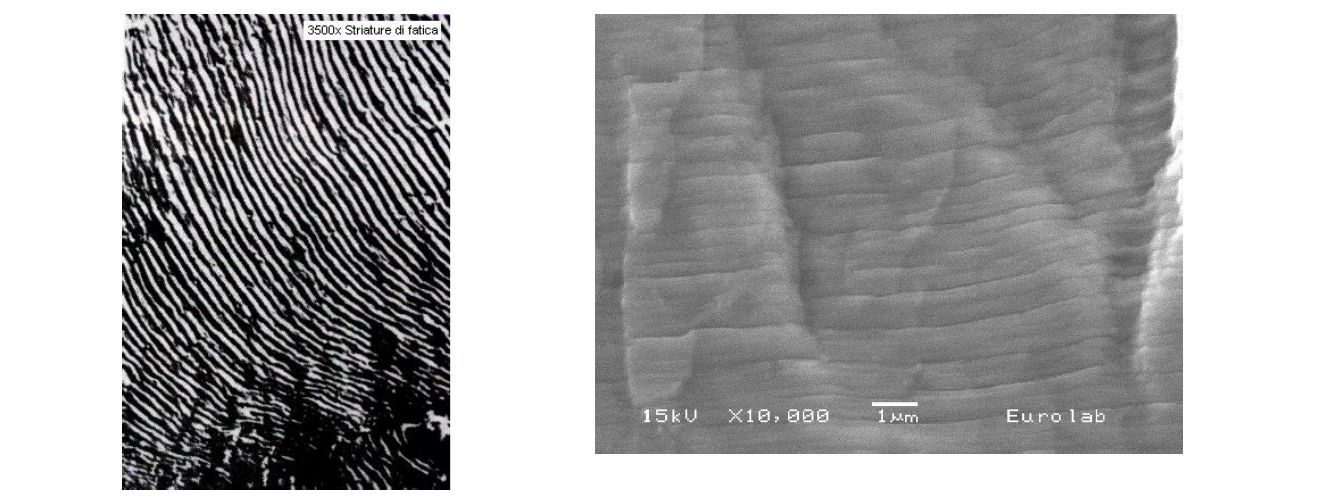
\includegraphics[width=0.3\linewidth]{immagini/screenshot010}
	\label{fig:screenshot010}
\end{figure}

			Sotto la validità delle proprietà booleane, mi posso ricondurre ad una somma di sezioni rettangolari, considerando l'inerzia totale come somma delle inerzie, per cui: 
			\[J_t = \dfrac{1}{3}\sum_il_i\delta^3_i\]
			\[ \tau = \dfrac{M_t}{J_t}\delta\]
			La tensione massima si valuterà invece tratto per tratto e nella formula ci andrà al denominatore l'inerzia totale dell'intera sezione, mentre al numeratore il valore dello spessore in quel tratto, per spessori variabili si tornerà invece alle formulazioni con $y$ esplicito: 
			\[ \tau_{xz} = -2\dfrac{M_t}{J_t}y \]
			Notare che una maggiore tensione si troverà su una sezione del tratto più spesso, perché in fin dei conti, il valore $\dfrac{M_t}{J_t}$ è null'altro che il coefficiente angolare di una retta che ha la stessa pendenza su tutta la sezione. \newline 
			
			Alcune sezioni notevoli:
			\[\begin{array}{ccc}
				\text{Sezione L} & \text{Sezione tubolare aperta} \\
				J_t = \dfrac{1}{3}(b+h)\delta^3 \hspace{0.2cm} \tau_{z,max} =\dfrac{3M_t}{(b+h)\delta^3}  & J_t = \dfrac{1}{3}(2\pi R)\delta^3\hspace{0.2cm}  \tau_{z,max} =\dfrac{3M_t}{(2\pi R)\delta^3}   
			\end{array}\]
			\[ \begin{array}{c}
				\text{Sezione C} \\
				J_t = \dfrac{1}{3}(2b+h)\delta^3 \hspace{0.2cm}  \tau_{z,max} =\dfrac{3M_t}{(2b+h)\delta^3} 
			\end{array}\]
		
		\textbf{{\Large Sezione sottile aperta pluriconnessa}}\newline
		\textit{La linea media non forma un percorso chiusa ma si biforca.}  
		\begin{figure}[H]
			\centering
			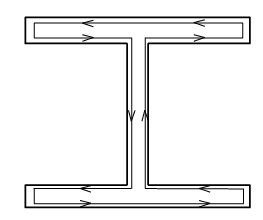
\includegraphics[width=0.3\linewidth]{immagini/screenshot011}
			\label{fig:screenshot011}
		\end{figure}
		
		Pratico lo stesso approccio appena portato a termine:
		\begin{enumerate}
			\item Si suddivide la sezione in porzione rettangolari \( J_{t,i} = \dfrac{1}{3}l_i\delta^3_i \)
			\item Si ripartisce il momento torcente tra i rettangoli \( \tau_{max,i} = \dfrac{M_{t,i}}{J_{t,i}}\delta_i\)
			\item Si ricavano le tensioni sul singolo rettangolo
		\end{enumerate}
		L’inerzia torsionale della sezione è data dalla somma delle inerzie dei
		singoli rettangoli:
		\[ M_t = \sum_i G\Theta J_{t,i} = G\Theta \sum_i J_{t,i} = G\Theta J_t\]
		\[ J_t = \sum_i J_{t,i} \]
		Ogni rettangolo è sottoposto ad una frazione del momento torcente
		proporzionale alla propria inerzia torsionale, ogni rettangolo si prende la sua quota di momento torcente in base a quanto è rigido:
		\[ M_{t,i} = M_t\dfrac{J_{t,i}}{J_{t}} \]
		Le tensioni tangenziali massime sono funzione dello spessore del
		rettangolo: massime nel rettangolo con spessore maggiore.
		\[ \tau_{max,i} = \dfrac{M_{t,i}}{J_{t,i}}\delta_i = \dfrac{M_t}{J_t}\delta_i \]
		Nelle sezioni pluriconnesse non è importante andare a capire quanto vale il momento torcente o la sua aliquota sul singolo tratto rettangolare, l'importante è conoscere lo spessore di ciascun termine, alla fine l'andamento a farfalla ha sempre la stessa pendenza su ciascun ramo: a spessori maggiori corrisponderanno sempre tensioni maggiori e si localizzeranno sull'estradosso. 	\newline 
			
		\textbf{{\Large Sezione cava a parete sottile}}\newline
		Si consideri una trave la cui sezione retta è caratterizzata da una linea media che sia una curva sufficientemente
		regolare nel piano o equivalentemente formata da archi di curva regolari. 
		
		Sotto le seguenti ipotesi:
		\begin{itemize}
			\item Spessore piccolo rispetto alla lunghezza della linea media \(\dfrac{\delta(s)}{a}<<1\)
			\item Funzione dello spessore continua \( a = \int_{l_m}ds\)
			\item Curvatura della linea media  piccola \(\dfrac{\delta(s)}{R}<<1\)
			\item Per sezioni generate da spezzate veridicità di tali condizioni a tratti \newline \( \left|\dfrac{d\delta(s)}{d}\right|<<1 \)
		\end{itemize}
		Vale quanto detto fin'ora, lungo lo spessore $\tau$ sarà costante, a maggior ragione se la sezione si chiude su se stessa.
		
\begin{figure}[H]
	\centering
	\label{fig:screenshot012}
	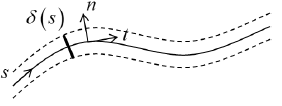
\includegraphics[width=0.5\linewidth]{immagini/screenshot012}
\end{figure}
		
		L’ipotesi di sottigliezza implica che le normali al bordo esterno a quello interno e alla linea media siano coincidenti
		in direzione: le tensioni tangenziali devono essere necessariamente orientate come $\hat{t}$ per rispettare l’equilibrio al
		contorno. \newline 
		
		Si immagini di tagliare la sezione chiusa con due code generiche, l'equilibrio a traslazione vedrà l'instaurarsi degli sforzi tangenziale uguali e contrari \newline \(\tau_1\delta_1\cdot 1 = \tau_2\delta_2\cdot 1 \), valendo a dire questo che la distribuzione delle tensioni $\tau$ genera un flusso di tensione costante:
		\[\tau\delta = q \Rightarrow \tau = \dfrac{q}{\delta}\]
\begin{figure}[H]
	\begin{flushright}
		\begin{tikzpicture} [>=latex]
			%		\draw [thin, help lines] (0,0) grid (15,15);
			%		\foreach \x in {0,...,15}
			%		\draw (\x cm,1pt) -- (\x cm,-1pt) node[anchor=north] {$\x$};
			%		\foreach \y in {0,...,15}
			%		\draw (1pt,\y cm) -- (-1pt,\y cm) node[anchor=east] {$\y$};
			%%% Solido
			\draw[thick] (1,11) -- (1,14) -- (3, 12) -- (3, 9) -- (1,11);
			\draw[thick] (8,1) -- (8,4) -- (6, 6) -- (6, 3) -- (8,1);	
			\draw[thick] (3,12) to[bend left = 100] (6,6);
			\draw[thick] (1,14) to[bend left = 100] (8,4);
			\draw[thick] (3,9) to[bend left = 100] (6,3);
			\draw[thick] (8.95,8) to[bend left=25] (8,1);
			%%% Corde
			\draw[thick, blue] (0,15) -- (4,11) node [pos = 1, right] {$c_1$};
			\draw[thick, blue] (5,7) -- (9,3) node [pos = 0, left] {$c_2$};
			%%% Vettori bassi
			\draw[->, thick, blue] (1.5,13.5) -- (1.5,12.5);
			\draw[->, thick, blue] (2.5,12.5) -- (2.5,11.5);
			%%% Vettori alti
			\draw[->, thick, blue] (1.5,13.5) -- (0.5,13.5);
			\draw[->, thick, blue] (2.5,12.5) -- (1.5,12.5);
			
			%%% Vettori bassi
			\draw[->, thick, blue] (6.5,5.5) -- (6.5,4.5);
			\draw[->, thick, blue] (7.5,4.5) -- (7.5,3.5);
			%%% Vettori alti
			\draw[->, thick, blue] (6.5,5.5) -- (7.5,5.5);
			\draw[->, thick, blue] (7.5,4.5) -- (8.5,4.5);
			%%% Vettori rossi
			\draw[->, thick, red] (2,13) -- (2,15) node [pos = 1, above] {$\tau_1\delta_1\cdot1$};
			\draw[->, thick, red] (7,5) -- (7,3) node [pos = 1, below] {$\tau_2\delta_2\cdot1$};
			%%% Dimensione 
			\draw[<->, thick, red] (10,1) -- (10,4) node [pos = 0.5, right] {1};
			\draw[dashed, thick, red] (8,4) -- (10,4);
			\draw[dashed, thick, red] (8,1) -- (10,1);	
		\end{tikzpicture}
	\end{flushright}
\end{figure}
		Se da una parte lo spessore cresce la tensione della parte opposta si riduce, in completa analogia idrodinamica, per una sezione stretta $\tau\uparrow$ mentre per una sezione larga $\tau\downarrow$: la tensione $\tau$ di dimostra così essere inversamente proporzionale allo spessore, al contrario delle sezioni aperte.\newline 
		
		Se si esprime l'equilibrio tra il momento torcente esterno e le azioni interne, questo diviene: 
		\[ M_0 = \oint_{l_m}\tau(s)\delta(s)h(s)ds = \tau(s)\delta(s)\oint_{l_m}h(s)ds = 0\]
		
\begin{figure}[H]
	\centering
	\label{fig:screenshot013}
	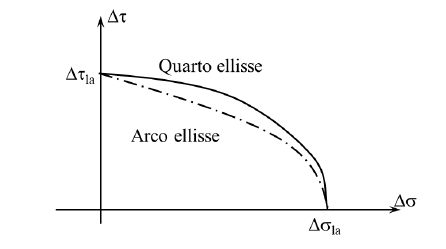
\includegraphics[width=0.5\linewidth]{immagini/screenshot013}
\end{figure}

		Dove $ h(s) $ è la distanza del polo dalla linea media, questa integrata sul percorso corrisponde proprio ad ottenere  il doppio dell'area sottesa dalla linea media stessa:
		\[{1\over2} \oint_{l_m}h(s)ds = \Omega_m \Rightarrow \oint_{l_m}h(s)ds = 2 \Omega_m\]
		E dunque l'equilibrio si può riscrivere: 
		\[ M_0 = \tau(s)\delta(s)\oint_{l_m}h(s)ds = \tau(s)\delta(s)2 \Omega_m = 0\]
		Giungendo infine ad: 
		\[ \tau(s) = \dfrac{M_0}{2\delta(s) \Omega_m}\]
		Lo stato tensionale così ipotizzato prende il nome di tensioni alla
		Bredt. \newline 
		
		Si ricordi anche questa essere una soluzione approssimata,	questo valore infatti rappresenta l’aliquota costante della distribuzione legata ad un momento $M_0$. D'altro canto l'andamento è costante lungo lo spessore, ma in realtà l'andamento è questo: 
		
\begin{figure}[H]
	\centering
		\begin{tikzpicture} [>=latex]
	%%%	Help Lines
%	\draw [thin, help lines] (0,0) grid (5,5);
%	\foreach \x in {0,...,5}
%	\draw (\x cm,1pt) -- (\x cm,-1pt) node[anchor=north] {$\x$};
%	\foreach \y in {0,...,5}
%	\draw (1pt,\y cm) -- (-1pt,\y cm) node[anchor=east] {$\y$};
	%%%	Disegno	
	\draw (0, 2) -- (4,2);
	\draw (0, 1) -- (4,1);
	\draw[pattern = horizontal lines, ultra thick] (1,1) -- (1,2) -- (3,2) -- (3.25, 1) --(1,1);
	\draw[thin, red] (3,2) -- (3,1);
	\node at (2,2.25) {$M_0$};
	\node[red] at (3.5, 1.5) {$M_1$};
\end{tikzpicture}
\end{figure}

		È tuttavia una piccola variazione lungo lo spessore di cui si considera il solo contributo costante che darà un contributo a torsione pari ad $M_0$: l'andamento reale a farfalla è matematicamente trascurabile e posso confondere perciò $M_t \approx M_0$. 
		
		\[M_t = M_0 + M_1 \approx M_0\]
		
		Si è così dimostrato come la tensione tangenziale per questo tipo di sezioni sia inversamente proporzionale allo spessore della parete e all'area racchiusa dalla linea media. \newline 
		
		Questa formulazione è estremamente potente perché da un andamento delle tensioni molto semplificato, è però applicabile \underline{ESCLUSIVAMENTE} alle sezioni in parete sottile chiuse. 
		
		
	
			
	
	\newpage
	{\Large \textbf{NOTE}}
%	\vfill
%\begin{tcolorbox}[height=4.5cm]
%	This box has a height of 4.5cm.
%\end{tcolorbox}

%DA DECOMMENTARE PER AVERE LA VERSIONE STAMPABILE A DUE PAGINE 	
%	\newpage
%		\null
%		\vfill
%\begin{tcolorbox}[height=4.5cm]
%	This box has a height of 4.5cm.
%\end{tcolorbox}
		\end{adjustwidth}

\end{document}
\newpage
\documentclass{article}
\usepackage[left=0.85in, right=0.85in, top=0.5in, bottom=0.95in]{geometry}
\usepackage[T1]{fontenc}
\usepackage[utf8]{inputenc}
\usepackage[italian]{babel}
\usepackage{graphicx}
\usepackage{wrapfig2}
\usepackage{amsmath, cancel}
\usepackage{amssymb}
\usepackage{cases}
\usepackage{gensymb} %simboli come ° = \degree  etc etc
\usepackage{subcaption}
\usepackage{pdfpages}
\usepackage{hyperref}
\hypersetup{
	colorlinks=true,
	linkcolor=blue,    
	urlcolor=blue,
	%pdfpagemode=FullScreen,
}
\urlstyle{same}
\usepackage{changepage}
\usepackage{lastpage, epstopdf}
\usepackage{fancyhdr}
\usepackage{tcolorbox}
%\usepackage{background}
\usepackage{tikz}
\usetikzlibrary{patterns}


%=======HEADER & FOOTER=======%
\def\lesson{Lezione N. 6}
\def\outcome{\textbf{Learning Outcomes:} Outcomes go here. }

\pagestyle{fancy}
\fancyhf{}
\renewcommand{\headrulewidth}{0pt}
\renewcommand{\footrulewidth}{1.4pt}
\lfoot{A.M. $\diamond$ \the\year}
\cfoot{Page \thepage}
\rfoot{\lesson}

%=======CORNELL STYLE FORMAT=======%
%\SetBgScale{1}
%\SetBgAngle{0}
%\SetBgColor{black}
%\SetBgContents{\rule{1pt}{0.85\paperheight}}
%\SetBgHshift{-1.6in}
%\SetBgVshift{-0.1in}

%=======CUSTOM BOXES=======%

\parindent 0ex

%=======BODY=======%
\begin{document}
	\setcounterpageref{secnumdepth}{0}
	\section*{Parte 6} %Date: \hrulefill}
%	\begin{tcolorbox}{\outcome}\end{tcolorbox}

\begin{adjustwidth}{2in}{} 
	
\textbf{{\Large De Saint Venant: Taglio}} \mbox{} \newline
		Si vuole studiare quella sollecitazione caratterizzata da un certo carico lineare risultante $T_y$ alla faccia terminale della sezione.
	
		Una forza $T_y$ così applicata porta ad avere per equilibrio, sulla faccia iniziale, la presenza contemporanea di una $T_y$ uguale e opposta. 
	
		Tali forze così applicate però sono in equilibrio? A traslazione si, a rotazione no.
	
		Si vedrà così l'insorgenza di una coppia, di un momento $M_x$ sulla faccia iniziale della trave. \newline 
	
		Non esiste sforzo di taglio senza l'insorgenza di flessione secondaria. La sollecitazione di taglio è sempre accompagnata da una sollecitazione di momento flettente. 
	
\begin{figure}[H]
	\centering
	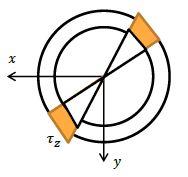
\includegraphics[width=0.5\linewidth]{immagini/screenshot001}
	\label{fig:screenshot001}
\end{figure}


		Un taglio è principale se viene applicato sulla direzione principale e porta a flessione retta; un taglio è deviato se non è applicato lungo una qualsivoglia direzione principale, si comporta come una composizione di tagli deviati e porterà a flessione deviata. \newline 
		
		Si studi l'equilibrio sulla faccia finale tramite il consolidato approccio alle tensioni: 
		\[ T_x = \int_A \tau_{zx}dA  = 0 \hspace{1cm}  T_y = \int_A \tau_{zy}dA  \hspace{1cm} N = \int_A\sigma_zdA = 0\]	
		Una qualunque distribuzione $\sigma_z$ che non sia banale genererebbe, seppur a risultante nulla in traslazione, un momento non nullo sulla faccia $S_l$, mentre invece si è imposto un momento flettente su tale faccia nullo, d'altronde per Cauchy, com'è che devono essere i vettori sulla faccia terminale per rispettare le condizioni al contorno? Uscenti dalla sezione finale, ma non essendo applicato alcuno sforzo normale, le uniche tensioni che applica $T_y$ sono delle $\tau_{zy}$.  \newline 
		
		Cosa risulta dall'equilibrio interno?
		\[
		\begin{cases}
			\begin{aligned}
				\frac{\partial \tau_{zx}}{\partial z} & =0 \\
				
				\frac{\partial \tau_{zy}}{\partial z} & =0 \\
				
				\frac{\partial \tau_{xz}}{\partial x} + \frac{\partial \tau_{yz}}{\partial y} + \frac{\partial\sigma_z}{\partial z} & =0 \\
			\end{aligned}
		\end{cases}
		\]
		Dalla $III$ equazione si vede che, se esistono delle $\tau_{zy}, \tau_{zx}$ la cui derivata è nulla, devono essere pari a \(\frac{\partial\sigma_z}{\partial z}\).
		
		Se si ipotizza una $\sigma_z$ costante lungo l'asse $z$ tale derivata è nulla e il problema sarebbe riconducibile al caso della flessione: con le stesse ipotesi ci si riconduce alle stesse soluzioni. 
		
		Ci si aspetta invece che $\sigma_z(z)\neq0$, variabile in $z$ perché, seppur in $S_l$ non ci sia momento, in $S_0$ esiste eccome, e cos'è che genera un momento flettente su quella faccia? Da cosa sono equilibrati gli $M_x$? Da delle tensioni normali $\sigma_z$!
		
		$\sigma_z$ esiste sulla faccia $S_0$ e non è vero che \(\frac{\partial\sigma_z}{\partial z} = 0\). \newline 
		
		Se si traccia il diagramma delle sollecitazioni
		
		
\begin{figure}[H]
	\centering
	\includegraphics[width=0.5\linewidth]{immagini/screenshot002}
	\label{fig:screenshot002}
\end{figure}

		Si nota che a seguito dell'applicazione $T_y$ si avrà un taglio costante su tutta la trave, una sollecitazione di momento flettente che non è più costante lungo tutta la trave, al contrario delle flessione retta; e una sollecitazione flessione con un momento flettente che non è più costante lungo tutta la trave ma linearmente variabile, con che legge varia? Attraverso le equazioni indefinite di equilibrio so ricondurmi ad un andamento simile:
		\[M^0_x=-T_yL\]
		Dove il segno meno tiene conto che il momento applicato è in verso orario anziché antiorario. \newline 
		
		Per sezione generica a quota $z$: 
		\[M_x=-T_y(L-z) =T_y(z-L) \]
		Che verifica inoltre la condizione per cui, se $z=L$:
		\[M^L_x=0\]
		
		Se il momento flettente ORA varia con la quota $z$, le tensioni $\sigma_z$, avranno sì andamento simile a quello del momento flettente, ma variabile proprio lungo la $z$.
		
		D'altronde, una volta che con De Saint Venant so ricavarmi alla generica sezione quanto valgono le caratteristiche della sollecitazione non ci sarà più bisogno di risolvere ogni volta il problema, userò quel valori ottenuti per ricavare le tensioni: attraverso le caratteristiche della sollecitazione per quella sezione costruirò con DSV la distribuzione di tensione su quella sezione, anche a partire dai valori numerici di momento, taglio e sforzo.
		
		Per flessione retta valeva: 
		\[\sigma_z = \dfrac{M_x}{I_x}y = \dfrac{T_y(z-L)}{I_x}y\]
		E il diagramma a farfalla diminuirà d'intensità lungo le sezioni.

\begin{figure}[H]
	\centering
	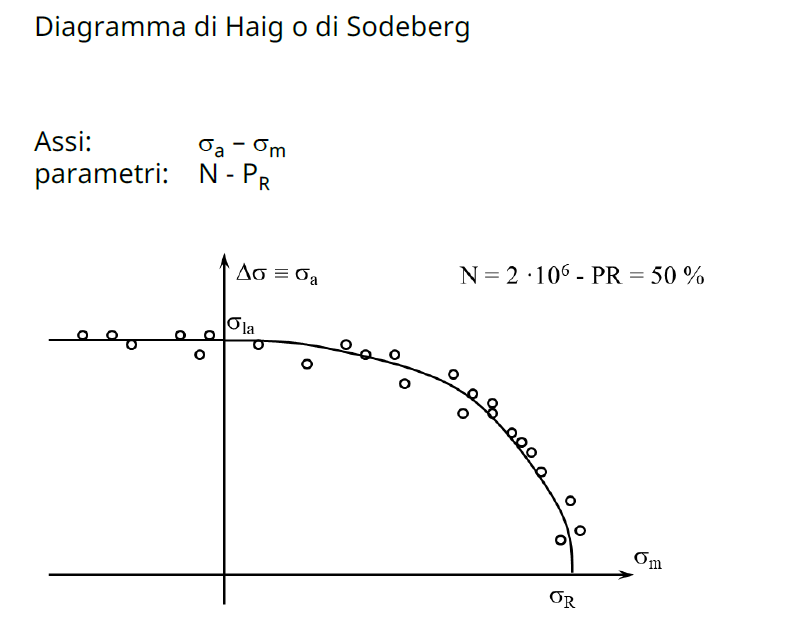
\includegraphics[width=0.5\linewidth]{immagini/screenshot003}
	\label{fig:screenshot003}
\end{figure}

		Si conferma così che che la tensione normale non è solo dipendente da $y$ ma anche da $z$.\newline 
		
		Il risultato di uno sforzo di taglio applicato all'estremo della trave genera tensioni normali variabili in $z$ ed $y$ e tensioni tangenziali, per la valutazione di queste ultime sorgono non pochi problemi da affrontare. \newline 
		
		La risultante del taglio cambia l'entità del valore della tensione e la sua tipologia in base alla sua retta d'azione.
		
		Per i momenti era d'interesse il solo asse dei momenti che tutt'al più poteva essere baricentrico, con lo sforzo normale invece in dipendenza che l'asse di applicazione fosse baricentrico o meno, generava trazione o pressoflessione. 
		
		Il taglio genera una casistica simile a quella della pressoflessione, sebbene con sia più il baricentro il punto d'interesse: se si sta considerando come prima ipotesi un taglio $T_y$ su asse principale d'inerzia (se così non fosse basterebbe una composizione lungo tali assi), l'importante è che l'asse delle linee di forza passi per un punto specifico chiamato centro di taglio $C_t$, qualora la forza passasse per questo centro di taglio le azioni che si stabilirebbero sarebbero esclusivamente di taglio, un \textbf{taglio puro}, qualora invece questa forza non passasse per questo centro di taglio, oltre alla generazione di sforzi di taglio, normali e flessionali, genererebbe anche delle azioni tangenziali di torsione. \newline 
		
		 Quando $T_y$ passa per un punto $C_t$ non c'è torsione.
		 
		 Il che si traduce nel dire che  torsione e taglio sono ortogonali in energia: le sollecitazioni di taglio non compiono lavoro virtuale con un possibile campo di spostamenti (deformazioni) associato alla torsione. \newline
		 
		 Nella pratica si ottengono le seguenti equazioni per le coordinate di $C_t$:
		 \[  x_t = {1\over T_y} \int_A\omega \cdot \left(\vec{\nabla}\cdot\vec{\tau}_z\right) = -{1\over I_x}\int_A\omega\cdot ydA \hspace{1cm} y_t = -{1\over I_y}\int_A\omega\cdot xdA\]
		 Entrambe dipendenti dalla funzione ingobbamento. 
		 
		 Si sfrutti qualche proprietà di questa funzione, noto che laddove la sezione è simmetrica o doppio simmetrica $\omega$ ha andamento simmetrico doppio simmetrico, questo si traduce nel dire che - ai fini del centro di taglio - se esiste un asse  di simmetria $C_t$ giace su tale asse, se esistono due assi di simmetria $C_t$ giace su entrambi gli assi, e come fa un punto a giacere su due rette? Vuol dire che è intersezione di queste, e qual è l'intersezione di due assi di simmetria? Il baricentro. 
		 
		 Qualora il centro di taglio non appartenesse agli assi di simmetria si vedrebbe l'applicazione di uno sforzo di torsione pari esattamente alla forza di taglio per la distanza tra la retta d'azione della forza ed il $C_t$: un momento torcente uniforme che si applica su tutta la trave. \newline 
		 
		 Che tensioni tangenziali genera una forza di taglio così orientata? Siccome non si riesce a risolvere questo problema in forma chiusa si applicherà un approccio semplificato con ipotesi altamente stringenti, accurato per sezioni in parete sottile e tutte le possibili combinazioni di tratti sottili (H, C, T, doppia T \dots) con applicazioni privilegiate per sezioni compatte con massa e area prossime al baricentro. 
		 
		 L'approccio sarà tanto più errato quanto più la sezione si inspessisce diventando frastagliata e irregolare, per cui tanto più è larga la sezione della direzione ortogonale al taglio, tanto più tali ipotesi perderanno validità.\newline 
		 
		 \textbf{HP}: Supponiamo di avere una sezione generica e di eseguire una suddivisione con una corda $b$ dividendo l'area in $A'$ ed $A''$ definisco poi i vettori $\hat{m} \perp b; \hat{l} \parallel b$. 
		 
\begin{figure}[H]
	\centering
	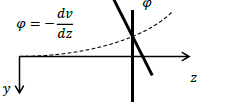
\includegraphics[width=0.5\linewidth]{immagini/screenshot004}
	\label{fig:screenshot004}
\end{figure}
		 
		 L'approssimazione sta nel dire che la distribuzione di $\tau$ lungo questa corda è una distribuzione di due componenti $\tau_{zm}\downarrow$ e $\tau_{zl}\rightarrow$ e dove più $\hat{m} \approx \hat{y}$ più la componente principale di tensione è la  $\tau_{zm}$ rispetto alla  $\tau_{zl}$. Inoltre più questi $\tau_{zm}$ sono principali, più la distribuzione reale è una distribuzione approssimabile ad un andamento continuo:
		 \[\tau_{zm} = {1\over b}\int_{B_1}^{B_2}\tau_{zm}ds\]
		 Più la sezione è sottile e più l'approssimazione è corretta: la distribuzione di tensioni sarà costante lungo l'ascissa curvilinea $l$ che si muove lungo la corda $b$. \newline 
		 
		 Si consideri una trave a sezione compatta e semplicemente connessa. Si ricordi poi come la $III$ equazione indefinita di equilibrio si possa scrivere: 
		 \[ \vec{\nabla}\cdot\vec{\tau}_z = -\dfrac{\partial \sigma_z}{\partial z} = -\dfrac{T_y}{I_x}y \]
		 Avere ora una divergenza non nulla implica avere delle linee di flusso non più chiuse ed avere linee di flusso aperte significa che lungo i percorsi - che ora avranno inizio e fine - si genereranno delle tensioni $\tau$ che varieranno lungo l'ascissa curvilinea. \newline 
		 
		 \item[$\rightarrow$] Integro direttamente $\tau_z$ che so lungo la corda essere costante:
		 \[ \int_{A'} \vec{\nabla}\cdot\vec{\tau}_z dA = \int_{\partial A'} \vec{\tau}_z \cdot \hat{m} ds + \underbrace{\int_{\partial A' -B_1B_ 2} \vec{\tau}_z \cdot \hat{m} ds}_\text{$0:\vec{\tau}_z\perp\hat{m}$ per le C.C.} = \int_{B_1}^{B_2} \vec{\tau}_z \cdot \hat{m} ds = \tau_{zm}b \]
		 \item[$\rightarrow$] Ma so che \( \vec{\nabla}\cdot\vec{\tau}_z = -\dfrac{T_y}{I_x}y\):
		 \[ \int_{A'} \vec{\nabla}\cdot\vec{\tau}_z dA = -\int_{A'}\dfrac{T_y}{I_x}ydA = -\dfrac{T_y}{I_x}S_x^{A'}\]
		 Allora necessariamente:
		 \[\tau_{zm}b = -\dfrac{T_y}{I_x}S_x^{A'} \]
		 \[ \tau_{zm} = -\dfrac{T_y}{I_x}\dfrac{S_x^{A'}}{b} \]
		 Tale formula prende il nome di \textbf{formula di Jourawski} ed è negativa se si prende in considerazione l'area superiore la corda. \newline 
		 
		 Non si sono però verificate nè compatibilità, nè congruenza, ebbene, non li soddisfa entrambe, non è una soluzione esatta, approssima però correttamente lo stato tensionale. \newline 
		 
		 La stessa formula si può ricavare anche per equilibrio. 
		 
\begin{figure}[H]
	\centering
	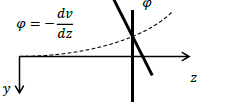
\includegraphics[width=0.3\linewidth]{immagini/screenshot004}
	\label{fig:screenshot004.2}
\end{figure}

		Che azioni interne si generano su una porzione della sezione? Applico lo studio all'area inferiore.

		La sollecitazione di taglio genera una $\tau_{zm}$, ma qual è il motivo per cui nascono queste tensioni sulla trave a seguito di una forza di taglio.
		
\begin{figure}[H]
	\centering
	\label{fig:screenshot005}
	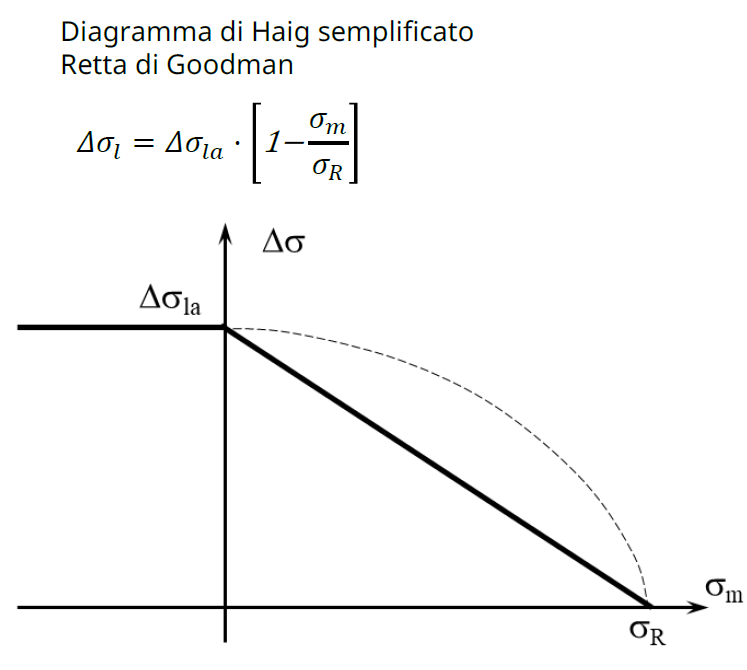
\includegraphics[width=0.5\linewidth]{immagini/screenshot005}
\end{figure}


		Separando le fibre del materiale, a seguito di una flessione, queste non occupano più la stessa posizione che occuperebbero se fossero state unite.
		
%IMAG qualitativa

		Quando le due fibre sono attaccate si trascinano l'un l'altra, quella inferiore trascina quella superiore facendogli compiere un percorso più lungo, c'è uno scorrimento dettato dall'azione tangenziale che le fibre si scambiano tra di loro, quando vengono separate tra le fibre non c'è più interazione, non si scambiano più nulla. \newline
		
		Il meccanismo fisico che mi porta ad avere delle tensioni nella sezione del taglio non è solo derivante dal fatto che la forza diviene adesso distribuita su quella sezione, ma anche dal fatto che l'azione che fa abbassare un estremo rispetto all'altro fa scorrere le fibre l'una con l'altra generando delle tensioni tangenziali, poi per equilibrio è logico che se esiste una $\tau$ su una faccia, ne esisterà un'altra uguale e opposta sull'altra faccia. 
		
		Ciò che si vede sulle facce quindi è in realtà l'equilibrio, l'azione del vettori nel piano $mz$ che è creato dallo scorrimento delle fibre, dal trascinamento tangenziale.  \newline 
		
		Si scriva così l'equilibrio in direzione $z$ delle azioni sul volume di sezione $A''$:
		\[ -\int_{A''}\sigma_zdA + \int_{A''}\left(\sigma_z + \dfrac{\partial\sigma_z}{\partial z}dz\right)dA - \int_{B_1}^{B_2} \tau_{zm} \cdot dz ds = 0 \]
		\[ \int_{B_1}^{B_2} \tau_{zm} \cdot ds = \int_{A''}\dfrac{\partial\sigma_z}{\partial z} \]
		\[ \tau_{zm} = {1\over b} \int_{A''}\dfrac{T_y}{I_x}ydA = \dfrac{T_y}{I_x}\dfrac{S_x^{A''}}{b}\]
		Tale formula è perfettamente equivalente a quella poco sopra ricavata, dove la differenza risiede nel fatto che è positiva e si è presa in considerazione l'area inferiore la corda. \newline 
		
		D'altro canto per le proprietà booleane delle aree vale: 
		\[ S_x^{A} = S_x^{A'} + S_x^{A''} = 0 \Rightarrow S_x^{A'} = -S_x^{A''}\]
		Se si considera l'area contenente $\hat{m}$ si usa il $+$, se si considera l'area rispetto alla quale esce $\hat{m}$ si una il $-$.\newline 
		
		La relazione che abbiamo scritto dipende dal valore del taglio, dal valore del momento d'inerzia (e quindi dalla distribuzione d'area), dalla corda e dal momento statico, quello che non compare da nessuna parte è il punto d'applicazione del taglio $T_y$, per cui, data una sezione generica, ciò che sto considerando sono solo le tensioni tangenziali alla Jourawski derivanti da una forza in direzione $y$, ma se questa risultante fosse applicata in un punti qualsivoglia della sezione, se ha direzione come $y$ e valore noto, genererà sempre quelle tensioni, cos'è allora che varia in dipendenza del punto di applicazione? Il fatto che solo una passerà per il $C_t$ e genererà solo quelle specifiche azioni tangenziali alla Jourawski, tutte le altre genereranno in più anche del momento torcente. \newline 
		
		\textbf{NB}: ricorda che i momenti statici $ S_x^{A',A''} $ sono i momenti statici calcolati NON rispetto al baricentro proprio di quella suddivisione, ma rispetto al baricentro dell'intera sezione. \newline
		
		Ora che con Jourawski si sono ricavate le $\tau_{zm}$ ci si chiede se le azioni che si sono trascurate, le $\tau_{zl}$, siano d'interesse o meno. 
		
		Sempre dalla $III$ equazione di equilibrio, se la l'operatore divergenza cambia variabili è lo stesso assicurata l'equivalenza delle derivate, per cui: 
		\[ \vec{\nabla}\cdot\vec{\tau}_z  -\dfrac{\partial \sigma_z}{\partial z} = 0\]
		\[ \dfrac{\partial \tau_{zl}}{\partial l} + \dfrac{\partial\tau_{zm}}{\partial m} + \dfrac{\partial\sigma_z}{\partial z} = 0\]
		Derivando per $l$ due volte ottengo: 
		\[ \dfrac{\partial^3 \tau_{zl}}{\partial l^3} + \dfrac{\partial^3\tau_{zm}}{\partial l^2\partial m} + \dfrac{\partial^3\sigma_z}{\partial l^2\partial z} = 0\]
		Ma derivando due volte rispetto ad $l$ il termine:
		\[\sigma_z =  \dfrac{T_y(z-L)}{I_x}y \rightarrow 0\]
		E dunque:
		\[ \dfrac{\partial^3 \tau_{zl}}{\partial l^3} = - \dfrac{\partial^3\tau_{zm}}{\partial l^2\partial m}\]
		L'ipotesi alla base del modello di Jourawski è che le $\tau_{zm}$ lungo la corda, sono costati, e cosa succede se derivo rispetto ad $l$ una grandezza costante rispetto ad $l$, che la sua derivata sarà nulla. 		
		\[ \dfrac{\partial^3 \tau_{zl}}{\partial l^3} = 0\]
		La tensione parallela alla corda allora potrà essere al più di secondo grado in $l$:
		\[ \tau_{zl} = al^2 + bl + c\]
		Con termini $a,b,c$ di volta in volta determinati tramite opportune condizioni al contorno. \newline 
		
		\textbf{{\Large Taglio in sezioni compatte simmetriche}} \newline 
		Come si traduce tutto ciò che è stato trattato fin'ora in termini applicativi? Su sezioni compatte e simmetriche la trattazione purtroppo produce qualche falla, ma quanto sono approssimati i risultati?
		
\begin{figure}[H]
	\centering
	\label{fig:screenshot006}
	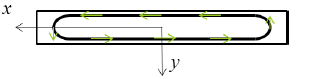
\includegraphics[width=0.2\linewidth]{immagini/screenshot006}
\end{figure}

		Essendo $y$ asse di simmetria e principale d'inerzia, se contiene $C_t$ e $G$, applicando una $T_y$ come in figura so che questa colpirà al $100\%$ il centro di taglio e sulla trave non si avrà nient'altro che un taglio puro: taglio con momento flettente. \newline 
		
		La tensione dipenderà così dalla quota $y$ piuttosto che da $x$, perché in questo caso è in funzione di $y$ che cambia il valore di $b$ ed $S_x$. 
		\[ \tau_{zm} = \tau_{zy} = \dfrac{T_y}{I_x}\dfrac{S_x^{A''}}{b}\]
		
		Come cambia $\tau$  in funzione che io mi trovi ai due apici della sezione? In questo tipo di sezione agli apici $b\rightarrow0$ e $S_x\rightarrow0$, ma a cosa si riconduceva il momento statico? Dalla definizione questo è l'area considerata per la distanza tra il baricentro dell'area considerata e l'asse rispetto al quale calcolo il momento statico stesso:
		\[S_x = A'' \cdot d(G_{A''}, x)\]
		Per entrambi gli apici, se si avesse soltanto $b\rightarrow0 \Rightarrow\tau\rightarrow\infty$ ma è assurdo perché $\tau$ è una grandezza fisica, si scopre così che all'apice superiore $S_x\rightarrow0$ molto più velocemente di $b$, in questo punto l'area sottesa dalla corda è tutta quella della sezione e $G_{A''}\equiv G$ ed ugualmente all'apice inferiore, molto più semplicemente è la stessa $A'' \rightarrow0$. \newline 
		
		Le tensioni così avranno un andamento che partirà dallo $0$ e ritornerà allo $0$, e non potevano fare altrimenti, d'altro canto delle tensioni tangenziali $\tau$ apicali non nulle avrebbero violato le condizioni al contorno di Cauchy. \newline 
		
		L'andamento delle tensioni tangenziali dipende da così da $S_x$ che ha un andamento quadratico/parabolico, per trovare il massimo di quest'andamento è sufficiente eseguire uno studio di funzione: 
		\[ {d\over dy}\tau_{zy} = {d\over dy}\left(\dfrac{T_y}{I_x}\dfrac{S_x^{A''}}{b}\right) = \dfrac{T_y}{I_x}\left( {1\over b}\dfrac{dS_x^{A''}}{dy} - \dfrac{S_x^{A''}}{b^2}\dfrac{db}{dy}\right) = 0\]
		Ma \( dS_x^{A''} = ybdy\) e così
		\[ \dfrac{T_y}{I_x}\left( {1\over b}\dfrac{dS_x^{A''}}{dy} - \dfrac{S_x^{A''}}{b^2}\dfrac{db}{dy}\right) = 0 \]
		Se e solo se è vero che:
		\[{1\over b}\dfrac{ybdy}{dy} = \dfrac{S_x^{A''}}{b^2}\dfrac{db}{dy}\]
		E dunque: 
		\[ y =  \dfrac{S_x^{A''}}{b^2}\dfrac{db}{dy}\]
		Viene fuori che la quota dove tale funzione è massima è la quota $y$ del baricentro, qualora, in corrispondenza di $G$, la corda $b$ abbia un valore massimo, o meglio qualora in corrispondenza di $G$ la derivata di $b$ rispetto ad $y$ sia nulla. 
		
		Se contemporaneamente alla quota baricentrica abbiamo anche una pendenza del fianco della sezione verticale allora quello sarà un punto di massimo dell'andamento del taglio. \newline 
		
		In questo caso oltre a notare che alla quota baricentrica la pendenza è verticale, si riporta anche l'andamento a farfalla delle $\sigma_z$. 
		
\begin{figure}[H]
	\centering
	\label{fig:screenshot007}
	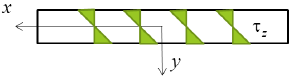
\includegraphics[width=0.5\linewidth]{immagini/screenshot007}
\end{figure}

		L'andamento delle tensioni $\tau_{yz}$ sulla corda generica non soddisfa però le condizioni al contorno, queste verificate solamente agli apici e agli estremi: ecco la prima forte approssimazione per sezione compatta. \newline 
		
		Per ripristinare le condizioni al contorno ho bisogno di una seconda componente di $\vec{\tau}$: dev'esserci anche un $\tau_{zx}$ tale che la combinazione lineare di $\tau_{xz}$ e $\tau_{zy}$ dia una tangenza al bordo della sezione la cui direzione determini un angolo $\gamma$. \newline
		
		La $III$ equazione di equilibrio, derivata una seconda volta rispetto ad $x$:
		\[\frac{\partial^2 \tau_{xz}}{\partial^2 x} + \cancel{\frac{\partial^2 \tau_{yz}(y)}{\partial x\partial y}} + \cancel{\frac{\partial\sigma_z(y,z)}{\partial x\partial z}}  =0\]
		\[ \frac{\partial^2 \tau_{xz}}{\partial^2 x} = 0\]
		Mi aspetto così una tensione $\tau_{xz}$ che varia al più secondo una legge lineare del tipo: 
		\[\tau_{xz} = \alpha x + \beta = 0\]
		Per risolvere il problema proposto ho bisogno di due condizioni al contorno , ricavabili queste dalle condizioni estremali su $B_1$ e $ B_2 $. 
		
\begin{figure}[H]
	\centering
	\label{fig:screenshot008.1}
	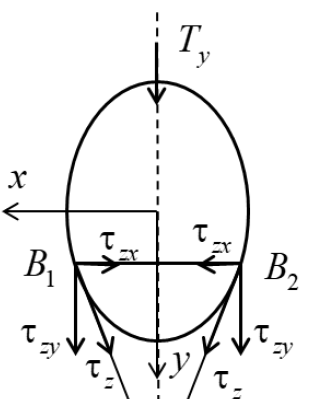
\includegraphics[width=0.2\linewidth]{immagini/screenshot008.1}
\end{figure}
		
		In $B_1$ $ \tau_{xz} $ è quella componente orizzontale tale che, combinata con la componente di Jourawski $ \tau_{yz} $, rende il vettore somma $\tau$ inclinato tangenzialmente al bordo, formando $\gamma$ con la verticale:
		\[ \begin{aligned}
			\tau_{xz}({b\over 2}, y) & = \tau_{yz}(y)\cdot \tan\gamma \\
			\tau_{xz}({-b\over 2}, y) & = -\tau_{yz}(y)\cdot \tan\gamma
		\end{aligned}\]
	 	\[ \tau_{xz} = -{2\over b}x\tau_{yz}\tan\gamma\]
	 	Nascono così queste azioni ortogonali all'asse $y$ con andamento a farfalla con massimo alle estremità e nullo sull'asse. 
	 	
\begin{figure}[H]
	\centering
	\label{fig:screenshot008.2}
	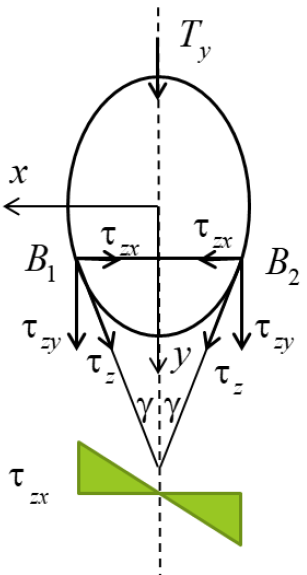
\includegraphics[width=0.2\linewidth]{immagini/screenshot008.2}
\end{figure}

		Chiudiamo la trattazione: quali sono le deformazioni associate alle azioni di taglio? Sicuramente si avranno degli scorrimenti angolari tra le facce che comporteranno certo abbassamento $d\eta$ al quale si aggiungerà un'inflessione dovuta al momento flettente $M_x$, che a meno che non sia un $M_x(z)$ la si sa già trattare: è ricavabile separatamente, sarebbe il contributo di abbassamento all'estremità di una mensola incastrata \(\dfrac{Ml}{EI}\) incontrato in \textit{meccanica dei solidi}, la rotazione dovuta alla flessione sarà così variabile lungo $ z $ in funzione del valore del momento flettente:
		\[ d\varphi = \dfrac{M_x}{EI_x}dz\]
		Il taglio applicato provoca anche un abbassamento dovuto allo slittamento di due facce della porzione di trave, pari ad una rotazione angolare per una lunghezza $dz$:
		\[d\eta = \Psi dz = \chi_y \dfrac{T_y}{GA}dz\]
		{\footnotesize (da meccanica dei solidi, parte 8 pag. 9)}\newline
		La rotazione angolare può essere valutata attraverso l'applicazione del principio dei lavori virtuali:
		\[ \Psi = \dfrac{T_y}{GA}\dfrac{A}{I_x^2}\int_{y_1}^{y_2}\dfrac{S_x^2}{b}\left(1 + {1\over 3}\tan^2\gamma\right)dy = \chi_y \dfrac{T_y}{GA} \] 
		Il fattore $\chi_y$ è chiamato fattore di taglio. \newline 
		
		\underline{In realtà} l'abbassamento alle estremità è dovuto all'inflessione della trave + un contributo dovuto al taglio, questo dovuto al fatto che le sezioni tra loro, a seguito dell'azione di taglio scorrono di una certa quantità l'una rispetto all'altra; l'ipotesi di Timoshenko e Bernoulli stanno a dire che questo scorrimento è o del tutto trascurabile, o da considerare, o da considerare così tanto che le sezioni oltre a scorrere, si ingobbano. \newline
		
		Oltre ad esserci scorrimento c'è anche una distorsione della sezione la quale si ingobbirà a causa del taglio.
		
		La sezione retta scorre, ma non subisce una distorsione angolare
		costante, poiché le tensioni tangenziali non lo sono. Negli estremi
		infatti le tensioni sono nulle, per cui l’angolo resta retto, causando
		un ingobbamento. 
		
\begin{figure}[H]
	\centering
	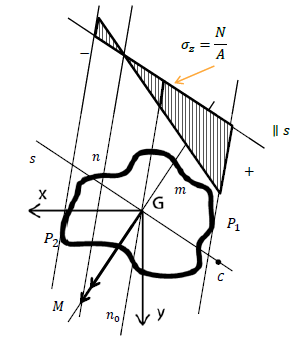
\includegraphics[width=0.15\linewidth]{immagini/screenshot008}
	\label{fig:screenshot008}
\end{figure}

		
		Naturalmente tutto ciò si valuterà laddove serva, in dipendenza che la trave sia snella non-snella o tozza, si valuteranno abbassamento e ingobbamento. 


\newpage

		\textbf{{\Large Taglio in sezioni compatte simmetriche: sezione circolare}} 
%\includepdf[pages={14}]{06_fcm_2022}
\end{adjustwidth}
\begin{figure}[H]
	\includegraphics[scale=0.75,page=13]{06_fcm_2022}
\end{figure}
\begin{adjustwidth}{2in}{}
		Dov'è minimo l'andamento? Dov'è massimo? Dov'è zero? Sapendo che la sezione è compatta con $T_y$ in quella direzione, l'andamento sarà nullo alle estremità e massimo al baricentro, inoltre, sapendo che se in corrispondenza del baricentro \({db\over dy}=0\), quello sarà un punto di massimo, a maggior ragione se la derivata è nulla a causa della tangenza verticale. \newline 
		
		Dov'è massima la $\tau$ di taglio? Sul baricentro. 
		
		In quale sezione della trave? Il taglio lungo la trave è costante, ma se $\tau$ dipende esclusivamente da $T$ e dalla sezione e la sezione è costante per DSV, se $T$ è uguale per ogni ascissa curvilinea allora mi aspetto un massimo uguale ovunque rispetto a $z$ per ogni sezione; rispetto ad $y$ sarà invece massimo dove è $y$ ad essere massima e rispetto ad $x$ non importa perché alla fine punti alla stessa quota $y$ hanno tutti lo stesso valore. \newline 
		
		Ci si ricordi però che nasce anche un momento flettente. Nel momento in cui si effettueranno le verifiche oltre a preoccuparsi del taglio, sarà importante anche la quota di momento flettente, ma ancor di più la loro composizione: dove si sommano i loro effetti? Qual è il punto più sollecitato? 
		
		La verifica si fa come sempre confrontando una $\sigma$ con una $\sigma_a$ ammissibile, dove la $\sigma$ sarà la massima tra tutti i punti da valutare. 
		
		In questo caso, ad esempio, dove sarà? 
		
		Il momento flettente sarà massimo secondo il diagramma:
		
\begin{figure}[H]
	\centering
	\begin{tikzpicture}
	\draw[thick] (0,0) -- (5,0);
	\draw[pattern = vertical lines] (0,0) -- (0,2) -- (5,0) -- (0,0);
\end{tikzpicture}
\end{figure}

		Mentre lo sforzo $\sigma_z$ sarà massimo lontano dall'asse, secondo questo diagramma:
		
\begin{figure}[H]
	\centering
	\begin{tikzpicture}
		\draw[thick] (0,-1) -- (3,-1);
		\draw[pattern = horizontal lines] (1,1) -- (3,1) -- (1,-1) --(1,1);
		\draw[pattern = horizontal lines] (1,-1)-- (0,-2) -- (1,-2) -- (1,-1);
	\end{tikzpicture}
\end{figure}

		Tutti i punti sollecitati a taglio sono sul $C_t\equiv G$, mentre quelli  a flessione sono quelli estremali, li valuto separatamente? 
		
		D'altronde dove è massimo uno è nullo l'altro e viceversa. \newline 
		
		\textbf{{\Large Taglio in sezioni sottili aperte}}  
\end{adjustwidth}
\begin{figure}[H]
\includegraphics[scale=0.75,page=14]{06_fcm_2022}
\end{figure}
\begin{adjustwidth}{2in}{} 

		Sezione sottile, ovunque a pendenza costante \({\partial b\over \partial y} = 0\), l'asse di simmetria lungo il quale si va ad applicare il taglio è $y$ come in figura, in questo modo incontro sicuramente $G\equiv C_t$ e il taglio è puro. \newline		

		Dove $y$ è la dimensione di $A'' $ mentre \( {h\over2} - y \over2\) è la distanza tra il baricentro di $A''$ e l'asse $x$ rispetto al quale si sta calcolando il momento statico. 
		
		L'asse baricentrico a pendenza verticale mi assicura che per il baricentro passerà il massimo della distribuzione di tensione. 
		
		La pendenza verticale inoltre implica che $\gamma=0$ ed esiste soltanto il contributo $\tau_{zy}$, esistono solo azioni tangenziali in direzione $y$, direzione del lato lungo della sezione.  
		
		Perché è così interessante la sezione sottile? Perché può essere combinata in più sezioni.  \newline 
		
\textbf{{\Large Taglio in sezioni sottili a doppia T}} \newline
		La sezione a doppia T ha sicuramente due assi di simmetrica e il baricentro si troverà così come in figura. \newline 
		
		Le due propaggini superiore e inferiore si chiamano \textbf{ali}, mentre la sezione che collega le due ali si chiama \textbf{anima} centrale. \newline 
		
		Con una $T_y$ applicata come in figura lo sforzo sarà di taglio puro.
		
\begin{figure}[H]
	\centering
	\label{fig:screenshot009}
	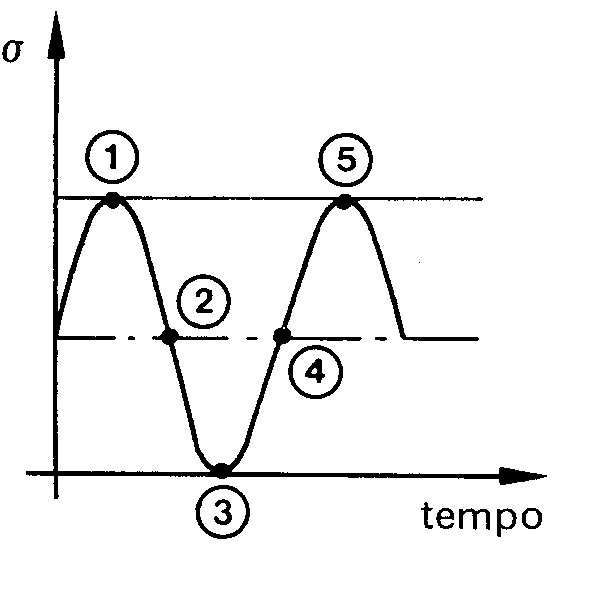
\includegraphics[width=0.3\linewidth]{immagini/screenshot009}
\end{figure}

		È una sezione che resiste ad alta flessione specifica, e com'è possibile generare una flessione? Con uno sforzo di taglio. \newline 
		
		Laddove la sezione risulti piccola, l'ipotesi di Jourawski è che tutto vada a collassare sulla linea media. 
		
		Si ragiona così lungo una linea media che passa per il centro, permettendo ciò di calcolare anche più agilmente i contributi $S_i, I_i$, perché si possono considerare i soli rettangoli componenti la sezione senza ripetizione o ridondanza di "elementini".\newline 
		
		Iniziamo a lavorare con Jourawski, mettiamoci su di una corda che taglia perpendicolarmente la linea media.
		
\begin{figure}[H]
	\centering
	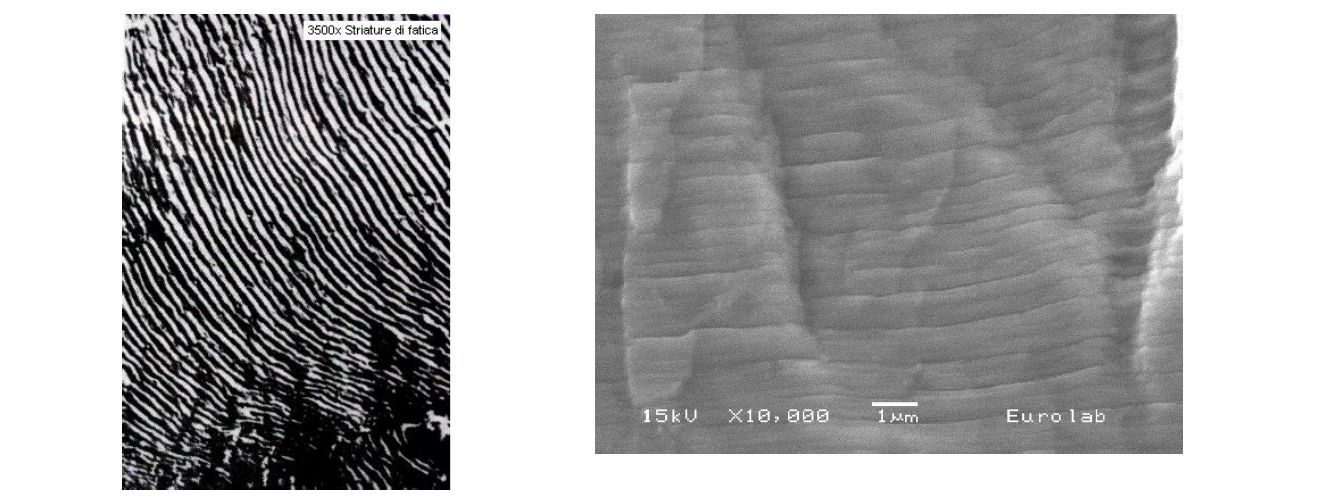
\includegraphics[width=0.3\linewidth]{immagini/screenshot010}
	\label{fig:screenshot010}
\end{figure}


		Il momento d'inerzia dell'intera sezione è: 
		\[ I_x = \dfrac{\delta H^3}{12} + 2\left[\dfrac{Bb^3}{12}  +Bb{H\over2}^2   \right]\]
		ricordi che il primo termine è quello che passa per l'asse $x$ e il successivo moltiplicato per 2 è il termine lontano dall'asse delle due ali? Ricordi che un momento d'inerzia calcolato per una superficie lontana dall'asse vale  \(A\cdot D^2\)? \newline 
		
		Il momento statico dell'area considerata vale: 
		\[S_x^{A''}= A'' \cdot d_xG'' + b\xi {H\over2}\]
		Considerando sempre la struttura coincidente sulla linea media (quindi senza portarsi dietro gli elementini ($b/2$). \newline 
		
		\[ \tau_{zm(zx)} = \dfrac{T_y}{I_x}\dfrac{S_x^{A''}}{b} = \dfrac{T_y}{I_x} {H\over2}\xi \]
		
		L'andamento della tensione parte da $0$ e cresce linearmente con $\xi$, il risultato è positivo e dunque segue in direzione in versore $\hat{m}$. 
		
		Per simmetria applico la stessa risoluzione alla mezzala opposta. 
		
\end{adjustwidth}
\begin{figure}[H]
\includegraphics[scale=0.75,page=16]{06_fcm_2022}
\end{figure}
\begin{adjustwidth}{2in}{} 

		Si salga adesso verso l'anima centrale, ora $ S_x^{A''} $ è data dal contributo intero dell'ala + il contributo del rettangolino $Y$ variabile questo con la quota $y$. \newline

		Il momento statico sarà dato dall'area per la distanza dai baricentri, e per le due figure può essere composto: 
		\[S_x^{A''}= A'' \cdot d_xG'' = Bb{H\over2} + \delta\left({H\over2} -y \right)\left({{H\over2} - y \over2} + y\right) = Bb{H\over2} + {\delta\over2}\left({H^2\over4}-y^2\right)\]
		Il risultato? Una $\tau_{zm}$ funzione di secondo grado. Dove sarà il massimo? La quota baricentrica ha una corda che garantisce \({\partial b\over \partial y} = 0\), quindi si avrà alla quota baricentrica. 
		\[ \tau_{zm(zy)}= \dfrac{T_y}{I_x}\dfrac{S_x^{A''}}{b} = \dfrac{T_y}{I_x\delta}\left[    \dfrac{bBH}{2} + {\delta\over2}\left({H^2\over4}-y^2\right) \right] \]

		Per l'ala superiore, varranno le stesse considerazioni ma prese con verso opposto. 		

		Tanto più è piccola la sezione, tanto più la situazione reale riflette quella qui riportata.  
		
		In analogia idrodinamica, la somma dei flussi entranti da sinistra e da destra, sarà uguale al flusso nell'anima:
		\[2\tau_{zx} = \tau_{zy}\delta\] 
		
		\textbf{{\Large Taglio in sezioni sottili a C}} \newline
\end{adjustwidth}
\begin{figure}[H]
\includegraphics[scale=0.75,page=17]{06_fcm_2022}
\end{figure}

\begin{figure}[H]
\includegraphics[scale=0.75,page=18]{06_fcm_2022}
\end{figure}
\begin{adjustwidth}{2in}{}  

		\textbf{{\Large Taglio in sezioni sottili chiuse}} \newline
		Nel caso di sezioni chiuse la soluzione con Jourawski si può applicare solo in presenza di assi di simmetria, in assenza di simmetria Jourawski non basta, perché al suo interno comparirebbero due incognite, una $\tau$ da un lato e da un altro indipendenti tra loro, dovrei aggiungere le condizioni di compatibilità ma questo mi comporterebbe un aggravio della matematica. \newline
		
		Con simmetria è possibile ricavare Jourawski esattamente come visto fin'ora, è come integrare un'ala superiore della doppia T.  
		
\begin{figure}[H]
	\centering
	\includegraphics[width=0.3\linewidth]{immagini/screenshot011}
	\label{fig:screenshot011}
\end{figure}
		
		
		Sfruttando la simmetria parto dall'asse della mezzala superiore e mi muovo ad esempio verso destra descrivendo la sezione d'interesse. 
		
		Ricordarsi che nelle sezioni laterali la larghezza della corda è doppi, perché sto prendendo due volte lo spessore. 
		
		Ci si riconduce sempre ad un andamento quadratico o lineare.
        \[ \begin{matrix}
        	S_x^{A'}= -2b\xi{H\over 2} &
        		\tau_{zm(zx)} = \dfrac{T_y}{I_x}{H\over2}\xi \\
        		S_x^{A''}= -Bb{H\over 2} - 2\delta\xi\left({H\over 2} - {\delta\over2}\right) &
        		\tau_{zm(zy)}=  \dfrac{T_y}{I_x}\dfrac{HB}{4} + \dfrac{T_y}{I_x}\xi \left({H\over 2} - {\delta\over2}\right)
        \end{matrix} \]
    	In completa analogia idrodinamica, se un flusso entra dall'alto, nei punti in cui $\tau=0$, questo si divide, discende e si ricongiunge in basso. 
    	\begin{figure}[H]
    		\centering
    		\includegraphics[width=0.5\linewidth]{immagini/screenshot012}
    		\label{fig:screenshot012}
    	\end{figure}
    	 
    	\newpage
    	\textbf{{\Large Determinazione del centro di taglio}} \newline
    	Sarà approfonditamente argomento di esercitazione. \newline 
    	
    	Se c'è un asse di simmetrica allo ra quello conterrà il $C_t$, se ci sono due assi di simmetria entrambi conterraneo il centro di taglio che si troverà a coincidere col baricentro.
    	
    	Generalmente si può dire che se ci sono due o più tratti di rettangoli e tutti questi concorrono in un unico punto senza fare percorsi multipli (sezioni a
    	T,L,V,K,X…), allora quello sarà il centro di taglio. \newline 
    	
    	Dal punti di vista pratico il $C_t$ non è altro che un punto di equilibrio tra le azioni esterne ed interne: dato il momento risultante dal carico $T$ applicato nel $C_t$ rispetto ad un polo qualunque $P^*$, allora \( \int\tau_{taglio}\) dovrà dare lo stesso momento. \newline 
    	
    	Se ci si mette su $P^*$ e si guarda l'azione del momento esercitata da $T_y$ questa pari a \(T_y\cdot x_t\). 
    	
    	Ora, è iù che noto come le azioni esterne debbano stare in equilibrio con le azioni interne, se si integrano perciò le $\tau$ che seguono le facce, queste daranno tre contributi di forza nelle seguenti direzioni $\leftarrow, \downarrow, \rightarrow$: il momento risultante di questa forza rispetto al polo scelto dovrà così dare esattamente \(T_y\cdot x_t\), è in questo modo che si potrà trovare il centro di taglio. 
    	
\begin{figure}[H]
	\centering
	\includegraphics[width=0.3\linewidth]{immagini/screenshot013}
	\label{fig:screenshot013}
\end{figure}

    	
    	\[ \begin{aligned}
    		T_x & = \int_{A^*}\tau_{xz}dA = \int_{0}^{B}\tau_{xz}bd\xi =\int_{0}^{B}\dfrac{T_yHB\xi}{2I_x}d\xi = \dfrac{T_yHB^2}{4I_x} \\
    		T_y & = \int_{A^**}\tau_{xz}dA
    	\end{aligned} \]
    	\[ TH = T_yd \Rightarrow d = {TH\over T_y} = \dfrac{H^2bB^2}{4I_x}\]
		
		\textbf{{\Large Osservazioni finali}} \newline
		\begin{itemize}
			\item Le tensioni tangenziali sono le medesime in ogni sezione della trave e seguono la direzione della linea media
			alla quale sono parallele;
			\item Verso
			e intensità sono dettate dalla formula di Jourawsky, con direzione dipendente dalla linea media, segue la linea media;
			\item Il
			flusso delle tensioni tangenziali varia ed è continuo lungo la linea media.
			
			Il prodotto $\tau\delta$ che per torsione a sezione chiusa era costante, ORA NON È PIÙ COSTANTE, tant'è che è $0$ alle estremità e massimo alla quota baricentrica;
			\item Le
			tensioni tangenziali sono massime in corrispondenza dell’asse neutro di tensione;
			\item A seguito della \( \vec{\nabla}\cdot\vec{\tau}\ne0\) le
			linee di flusso sono curve aperte alle cui estremità c'è flusso nullo e dunque tensione nulla;
			\item Se i fianchi sono rettilinei a maggior ragione varrà \( \partial b\over\partial y = 0\) e $\tau$ sarà massima sulla quota baricentrica;
			\item La trattazione non si modifica se l’asse principale y non è di simmetria.
		\end{itemize}
		
		
			
		
		 
		 
		 
		 

		


		
		
	
	
		
		
	
			
	
	\newpage
	{\Large \textbf{NOTE}}
%	\vfill
%\begin{tcolorbox}[height=4.5cm]
%	This box has a height of 4.5cm.
%\end{tcolorbox}

%DA DECOMMENTARE PER AVERE LA VERSIONE STAMPABILE A DUE PAGINE 	
%	\newpage
%		\null
%		\vfill
%\begin{tcolorbox}[height=4.5cm]
%	This box has a height of 4.5cm.
%\end{tcolorbox}
		\end{adjustwidth}

\end{document}				
		\end{document}
